%-------------------------------------------------------------------------------
%                      Template Naskah Skripsi
%               	Berdasarkan format JTETI FT UGM
% 						(c) @gunturdputra 2014
%-------------------------------------------------------------------------------

%Template pembuatan naskah skripsi.
\documentclass{jtetiskripsi}

%Untuk prefiks pada daftar gambar dan tabel
\usepackage[titles]{tocloft}
\renewcommand\cftfigpresnum{Gambar\  }
\renewcommand\cfttabpresnum{Tabel\   }

%Untuk hyperlink dan table of content
\usepackage{hyperref}
\newlength{\mylenf}
\settowidth{\mylenf}{\cftfigpresnum}
\setlength{\cftfignumwidth}{\dimexpr\mylenf+2em}
\setlength{\cfttabnumwidth}{\dimexpr\mylenf+2em}

%Untuk Bold Face pada Keterangan Gambar
\usepackage[labelfont=bf]{caption}
%Untuk caption dan subcaption
\usepackage{caption}
\usepackage{subcaption}

%pdf
\usepackage{pdfpages}

%table
\usepackage{graphics}

\usepackage{wrapfig}

\usepackage{natbib}
\setlength\bibhang{12mm}


%-----------------------------------------------------------------
%Disini awal masukan untuk data proposal skripsi
%-----------------------------------------------------------------
\titleind{Rancang Bangun Sistem Informasi Monitoring Kegiatan Belajar Mengajar menggunakan
\emph{Web Service} SIAKAD Di Rumpun Matematika FMIPA UNJ}

\fullname{Aldi Rahmansyah}

\idnum{3145161324}

\approvaldate{}

\degree{Sarjana Ilmu Komputer}

\yearsubmit{2021}

\program{Ilmu Komputer}

\dept{Ilmu Komputer}

\firstsupervisor{Med Irzal, M.Kom.}
\firstnip{}

\secondsupervisor{Ir. Fariani Hermin Indiyah, M.T}
\secondnip{}

%hypenation

\hyphenation{
me-ngum-pul-kan
ma-su-kan
DE-VE-LOP-MENT
Re-trie-ved
ke-se-jah-te-ra-an
di-la-ku-kan
sub-me-nu
pe-nam-ba-han
meng-gam-bar-kan
me-ngun-tung-kan
meng-gu-na-kan
di-gu-na-kan
per-ngem-ba-ngan
bra-in-wa-re
KOP-MA
di-ja-lan-kan
ke-wa-ji-ban
ser-ver
Mul-ti-pur-pose
XAM-PP
Mul-yo-no
pe-rang-kat
mem-pro-ses
me-la-ku-kan
ke-wa-jib-an
me-ru-pa-kan
di-bu-tuh-kan
pe-ni-lai-an
ber-kua-li-tas
a-kan
se-dang-kan
kar-ya-wan
di-per-gu-na-kan
sub-class
ser-vi-ce
con-trol-ler
me-nun-juk-kan
peng-ak-ses-an
RESTful
di-pro-ses
}

%-----------------------------------------------------------------
%Disini akhir masukan untuk data proposal skripsi
%-----------------------------------------------------------------

\begin{document}

\cover

%!TEX root = ./template-skripsi.tex
\chapter*{\centering{\large{LEMBAR PERSETUJUAN}}}
\thispagestyle{empty} {\bf }Dengan ini saya mahasiswa Fakultas
Matematika dan Ilmu Pengetahuan Alam, Universitas Negeri Jakarta

\vskip3mm

\begin{tabular}{ll}
  Nama & : Aldi Rahmansyah \\
  No. Registrasi & : 3145161324 \\
  Program Studi & : Ilmu Komputer \\
  Judul & :  Rancang Bangun Sistem Informasi Monitoring Kegiatan \\ & \hspace{0.2cm} Belajar Mengajar menggunakan \emph{Web Service} Di Rumpun \\ & \hspace{0.2cm} Matematika FMIPA UNJ
\end{tabular}

\vskip3mm

%\noindent \hskip10mm Menyatakan bahwa skripsi ini telah siap diajukan untuk sidang skripsi.
\begin{center}
Menyatakan bahwa skripsi ini telah siap diajukan untuk sidang skripsi.
\end{center}



\begin{center}
\vskip3mm

Menyetujui,

\vskip3mm
\begin{spacing}{1.25}

\begin{tabular}{ccc}
  \hskip-2mm Dosen Pembimbing I & \qquad \qquad \qquad \qquad \qquad & \hskip-6mm Dosen Pembimbing II \\
   &  &  \\
   &  &  \\
   &  &  \\
   &  &  \\
  \hskip-2mm \underline{\textbf{Med Irzal, M.Kom.}} &  & \hskip-6mm \underline{\textbf{Ir. Fariani Hermin Indiyah, M.T.}} \\
  \hskip-2mm NIP. 19770615 200312 1 001 &  & \hskip-6mm NIP. 19600211 198703 2 001	 \\
\end{tabular}
\end{spacing}
\end{center}
\vskip3mm
\begin{center}
Mengetahui, \\
Koordinator Program Studi Ilmu Komputer
\end{center}
\begin{spacing}{1.25}
{ \ }
\\
\\
{ \ }\begin{center}
\underline{\textbf{Ir. Fariani Hermin Indiyah, M.T.}} \\
{NIP. 19600211 198703 2 001}
\end{center}
\end{spacing} 
%\chapter*{\centering{\large{\thesisapprovalname}}}
\thispagestyle{empty} {\bf }
\vspace{-0.5cm}
\begin{center}
	\textbf{Perancangan Sistem Informasi Koperasi Serba Usaha Berbasis \emph{Website} Pada Lembaga Koperasi Mahasiswa Universitas Negeri Jakarta}
\end{center}

\vspace{1mm}
\vskip 1.5mm \noindent
\begin{tabular}{ll}
	\hskip-2mm Nama & : Muhammad Yan Handoko \\
	\hskip-2mm No. Registrasi & : 3145143620 \\
\end{tabular}


\vskip2mm

\noindent \begin{flushleft}
	\begin{tabular}{llcc}
		
		& \hskip15mm Nama & Tanda Tangan & Tanggal \\
		
		\hskip-1cm Penanggung Jawab &  &  &  \\
		\hskip-1cm Dekan & : Prof. Dr. Suyono, M.Si. & ............... & ............. \\
		& \hskip3mm NIP. 19671218 199303 1 005 &  &  \\
		\hskip-1cm Wakil Penanggung Jawab &  &  &  \\
		\hskip-1cm Wakil Dekan Bidang Akademik & : Dr. Muktiningsih, M.Si. & ............... & ............. \\
		& \hskip3mm NIP. 19640511 198903 2 001 &  &  \\
		\hskip-1cm Ketua & : Ir. Fariani Hermin I, M.T. & ............... & ............. \\
		& \hskip3mm NIP. 19600211 198703 2 001 &  &  \\
		\hskip-1cm Sekretaris & : Ari Hendarno, S.Pd, M.Kom & ............... & ............. \\
		& \hskip3mm NIDK. 8857650017 &   &  \\	
		\hskip-1cm Penguji Ahli & : Med Irzal, M.Kom. & ............... & ............. \\
		& \hskip3mm NIP. 19750925 200212 2 002 &  &  \\
		\hskip-1cm Pembimbing I & : Ratna Widyati, S.Si, M.Kom. & ............... & ............. \\
		& \hskip3mm NIP. 19750925 200212 2 002 &  &  \\		
		\hskip-1cm Pembimbing II & : Drs. Mulyono, M.Kom. & ............... & ............. \\
		& \hskip3mm NIP. 19660517 199403 1 003 &  &  \\
	\end{tabular}
\end{flushleft}

\vskip1mm

\noindent Dinyatakan lulus ujian skripsi tanggal: 18 Februari 2019


%\chapter*{\centering{\large{LEMBAR PERNYATAAN}}}

Saya menyatakan dengan sesungguhnya bahwa skripsi dengan judul 	\textbf{Perancangan Sistem Informasi Koperasi Serba Usaha Berbasis \emph{Website} Pada Lembaga Koperasi Mahasiswa Universitas Negeri Jakarta} yang disusun sebagai syarat untuk memperoleh gelar Sarjana komputer dari Program Studi Ilmu Komputer Universitas Negeri Jakarta adalah karya ilmiah saya dengan arahan dari dosen pembimbing.

Sumber informasi yang diperoleh dari penulis lain yang
telah dipublikasikan yang disebutkan dalam teks skripsi ini, telah dicantumkan dalam Daftar Pustaka sesuai dengan norma, kaidah dan etika penulisan ilmiah.

Jika dikemudian hari ditemukan sebagian besar skripsi ini bukan hasil karya saya sendiri dalam bagian-bagian tertentu, saya bersedia menerima sanksi pencabutan gelar akademik yang saya sanding dan sanksi-sanksi lainnya sesuai dengan peraturan perundang-undangan yang berlaku.

\vspace{.5cm}

\begin{tabular}{p{7.5cm}c}
	&Jakarta, 18 Ferbruari 2019\\
	&\\
	&\\
	&\\
	&Muhammad Yan Handoko
\end{tabular}

%-----------------------------------------------------------------
%Disini awal masukan Acknowledment
%-----------------------------------------------------------------
%\acknowledgment
%\begin{flushright}
%	\emph{Untuk Bapak dan Mama.}
%\end{flushright}
%-----------------------------------------------------------------
%Disini awal masukan untuk Prakata
%-----------------------------------------------------------------

\preface
\begin{onehalfspace}
Puji dan syukur penulis panjatkan kepada Allah SWT atas segala rahmat, berkah dan hidayah-Nya sehingga penulis dapat menyelesaikan proposal skripsi yang berjudul "Rancang Bangun Sistem Informasi Monitoring Kegiatan Belajar Mengajar Menggunakan \textit{Web Service} Di Rumpun Matematika FMIPA UNJ" dengan baik. Proposal skripsi ini dibuat dengan tujuan untuk memenuhi salah satu syarat memperoleh gelar Sarjana Komputer.  

Dalam proses pembuatan proposal skripsi ini, penulis mendapat banyak bantuan dan dorongan. Oleh karena itu, penulis ingin menyampaikan rasa terima kasih kepada Bapak Med Irzal, M.Kom selaku Dosen Pembimbing I dan Ibu Ir. Fariani Hermin Indiyah, M.T selaku Dosen Pembimbing II yang telah membimbing, mengarahkan, mengoreksi, serta memberikan berbagai saran dan masukan yang sangat bermanfaat dalam penyusunan proposal skripsi ini.

Dalam penyusunan proposal skripsi ini, penulis menyadari bahwa proposal skripsi yang telah dibuat ini masih sangat jauh dari kata sempurna dengan segala keterbatasan ilmu dan pengetahuan penulis sendiri. Baik dari segi penulisan, materi, dan bahasa. Oleh karena itu, penulis sangat membutuhkan kritik dan saran untuk dijadikan sebagai pembelajaran dan untuk membantu penulis menjadi lebih baik lagi kedepannya.

Akhir kata, penulis berharap agar proposal yang telah dibuat ini dapat memberikan manfaat kepada semua pihak, khususnya penulis sendiri. Penulis juga berharap ditulisnya proposal skripsi ini dapat menjadi motivasi dan memberikan semangat bagi rekan-rekan yang sedang dan akan menyusun proposal skripsi. Semoga Allah SWT senantiasa membalas kebaikan semua pihak yang telah membantu penulis dalam menyusun proposal skripsi ini.
\end{onehalfspace}
\vspace{.5cm}

\begin{tabular}{p{7.5cm}c}
	&Jakarta, 2 Juni 2021\\
	&\\
	&\\
	&\\
	&\\
	&\textbf{Penulis}
\end{tabular}


%-----------------------------------------------------------------
%Disini awal masukan Intisari
%-----------------------------------------------------------------
%\begin{abstractind}
%\textbf{MUHAMMAD YAN HANDOKO}. 	\textbf{Perancangan Sistem Informasi Koperasi Serba Usaha Berbasis \emph{Website} Pada Lembaga Koperasi Mahasiswa Universitas Negeri Jakarta}. Skripsi. Fakultas Matematika dan Ilmu Pengetahuan Alam, Universitas Negeri Jakarta. 2019. Di bawah bimbingan Ratna Widyati, S.Si, M.Kom dan Drs. Mulyono, M.Kom.
%\vskip1cm
	
%Koperasi Mahasiswa Universitas Negeri Jakarta (KOPMA UNJ) merupakan organisasi kemahasiswaan tingkat universitas yang bergerak dalam bidang perkoperasian. KOPMA UNJ merupakan koperasi serba usaha, yang tujuan utamanya adalah menyejahterakan anggota koperasi. Aspek perkoperasian yang dijalankan KOPMA UNJ adalah simpanan dan usaha. Pada prosesnya, pengelolaan dana simpanan akan digunakan untuk pembelian barang usaha yang pada akhirnya akan menghasilkan keuntungan untuk anggota yang disebut sisa hasil usaha (shu). Skripsi ini bertujuan untuk membangun sistem informasi KOPMA UNJ berbasis \textit{website} agar memudahkan pengurus KOPMA UNJ dalam mengelola dana simpanan dan usaha koperasi, serta agar anggota KOPMA UNJ dapat mengetahui transparansi dana simpanan yang mereka bayarkan kapanpun dan dimanapun. Sistem informasi KOPMA UNJ berbasis \textit{website} dikembangkan menggunakan metode pengembangan perangkat lunak (\textit{system development life cycle}) model \textit{spiral}. Model \textit{spiral} memiliki 4 tahapan pengembangan, yaitu analisis kebutuhan, desain sistem, implementasi, dan \textit{maintenance}. Sistem informasi KOPMA UNJ dibangun menggunakan \textit{framework codeigniter} untuk bagian \textit{back-end} dan \textit{framework bootstrap} untuk tampilan \textit{user} \textit{front-end}. \textit{User} yang ada pada sistem informasi KOPMA UNJ berjumlah 3, yaitu \textit{admin} yang dapat mengelola seluruh data simpanan dan usaha, anggota yang dapat mengetahui transparansi seluruh data, dan pengawas yang dapat mengelola data penilaian.
	
%	\bigskip
%	\noindent
%	\textbf{Kata kunci :} \textit{Webite}, sistem informasi, model \textit{spiral}, \textit{framework codeigniter}, \textit{framework bootstrap}, koperasi, simpanan, usaha.
%\end{abstractind}

%\begin{abstracteng}

%\textbf {MUHAMMAD YAN HANDOKO}. \textbf {Designing a Website-Based Multipurpose Cooperative Information System at the Koperasi Mahasiswa Universitas Negeri Jakarta}. Thesis. Faculty of Mathematics and Natural Sciences, State University of Jakarta. 2019. Supervised by Ratna Widyati, S.Si, M.Kom and Drs. Mulyono, M.Kom.
%\vskip1cm

%Koperasi Mahasiswa Universitas Negeri Jakarta (KOPMA UNJ) is a university-level student organization engaged in cooperatives. KOPMA UNJ is a multi-business cooperative, where the main goal is for cooperative member's prosperity. The cooperative aspects carried out by KOPMA UNJ are savings and business. For the process, the management of deposit funds will be used for purchasing business goods where will give benefits for members called sisa hasil usaha (shu). This thesis aims to build a website-based KOPMA UNJ information system in order to make it easier administrators of KOPMA UNJ to manage savings and cooperative business funds, and also for members of KOPMA UNJ will know the transparency of their deposit funds they have paid. Website-based KOPMA UNJ information system have been developed using a spiral model software development (system development life cycle) method. The spiral model have 4 stages of development, there are needs analysis, system design, implementation, and maintenance. The KOPMA UNJ information system was built using the framework codeigniter for the back-end and framework bootstrap for user front-end display. There are three users in the KOPMA UNJ information system, those are 'admin' where can manage all deposit and business data, 'members' where can find out the transparency of all data, and 'supervisors' where can manage the assesment data.

%\bigskip
%\noindent
%\textbf {Keywords:} Website, information system, spiral model, framework codeigniter, framework bootstrap, cooperative, savings, business.
%\end{abstracteng}

%-----------------------------------------------------------------
%Disini akhir masukan Intisari
%-----------------------------------------------------------------
%-----------------------------------------------------------------

%-----------------------------------------------------------------
%Disini akhir masukan untuk muka skripsi
%-----------------------------------------------------------------


\tableofcontents 
\addcontentsline{toc}{chapter}{DAFTAR ISI}
\listoffigures
\addcontentsline{toc}{chapter}{DAFTAR GAMBAR}
\listoftables
\addcontentsline{toc}{chapter}{DAFTAR TABEL}

\begin{counterpage}
\end{counterpage}
%Disini awal masukan untuk Bab
%-----------------------------------------------------------------
%!TEX root = ./template-skripsi.tex
%-------------------------------------------------------------------------------
% 								BAB I
% 							LATAR BELAKANG
%-------------------------------------------------------------------------------

\chapter{PENDAHULUAN}

\section{Latar Belakang Masalah}
	Tri Dharma Perguruan Tinggi adalah tiga pilar dasar pemikiran yang harus ada pada semua aspek di dalam sebuah perguruan tinggi mulai dari mahasiswa, dosen dan berbagai civitas akademika yang terlibat. Tri Dharma Perguruan Tinggi terdiri dari 3 poin, yaitu Pendidikan dan Pengajaran, Penelitian dan Pengembangan, dan Pengabdian Kepada Masyarakat.

	Kegiatan belajar mengajar adalah suatu kegiatan yang merupakan bagian dari salah satu isi Tri Dharma Perguruan Tinggi yang merupakan pendidikan dan pengajaran. Kegiatan belajar mengajar dijalankan oleh dua pihak, yaitu dosen dan mahasiswa. Keduanya merupakan faktor yang sangat berpengaruh dalam berhasilnya suatu kegiatan belajar mengajar. Dosen dan mahasiswa merupakan komponen penting dalam suatu sistem pembelajaran di perguruan tinggi dimana peran, tugas, dan tanggung jawab seorang dosen terutama dalam sebuah proses pembelajaran merupakan hal yang sangat penting dalam mewujudkan tujuan dari satu pilar Tri Dharma Perguruan Tinggi. Dalam melaksanakan kegiatan belajar mengajar perlu dilakukan pemantauan dan evaluasi untuk memastikan pelaksanaan kegiatan belajar mengajar mencapai tujuan yang diinginkan dan sesuai dengan standar yang ditetapkan oleh perguruan tinggi.

	Monitoring merupakan kegiatan pemantauan yang dilakukan untuk mengetahui proses kegiatan Belajar Mengajar yang dilakukan oleh dosen. Sedangkan evaluasi merupakan hasil akhir dari monitoring yang dilakukan selama proses Kegiatan Belajar Mengajar yang telah dilaksanakan selama satu semester. Monitoring dan evaluasi kegiatan belajar mengajar adalah tugas dari Tim Penjamin Mutu. Kegiatan ini dilakukan dengan tujuan untuk memastikan Kegiatan Belajar Mengajar yang disampaikan oleh dosen menerapkan aturan dan standar yang telah diterapkan oleh perguruan tinggi serta sesuai dengan Rencana Pembelajaran Semester (RPS).

	Seiring berkembangnya teknologi, sistem informasi dapat mempermudah berbagai kegiatan untuk menghasilkan informasi sebagai penunjang pengambilan keputusan dan mempermudah penyelesaian suatu masalah dan meningkatkan kinerja berbagai aktivitas. Penggunaan sistem informasi juga dapat dimanfaatkan pada berbagai macam aktivitas akademik pada sebuah perguruan tinggi seperti aktivitas kegiatan belajar mengajar beserta monitoring dan evaluasinya.

	Pandemi COVID-19 yang terjadi pada tahun 2020 dan masih berjalan hingga 2021 ini juga menyebabkan berubahnya kegiatan belajar mengajar yang sebelumnya dilakukan tatap muka di dalam ruang kelas menjadi daring atau \textit{online}. Dilakukannya kegiatan belajar mengajar menjadi daring menyebabkan sistem presensi dan pemantauan kelas manual yang menggunakan kertas tidak dapat lagi digunakan sehingga universitas yang masih menggunakan sistem manual terpaksa menggunakan solusi daring sementara seperti Google Form, Microsoft Form, atau tetap melakukan presensi dengan manual menggunakan file excel. Penggunaan form daring tersebut tentunya tidak efisien dikarenakan form-form tersebut tidak terintegrasi dalam satu sistem sehingga dibutuhkan suatu sistem informasi yang dapat memfasilitasi jalannya kegiatan belajar mengajar daring dan sekaligus mempermudah pemantauan kegiatan belajar mengajar tersebut.

	Pada Fakultas Matematika dan Ilmu Pengetahuan Alam (FMIPA) UNJ, kegiatan belajar mengajar dipantau melalui formulir 05 dan 06 oleh Tim Penjamin Mutu tingkat Program Studi yang selanjutkan diserahkan kepada Gugus Penjamin Mutu FMIPA UNJ. Dalam menjalankan kegiatan belajar mengajar, mahasiswa akan mengambil formulir 05 dan 06 dari ruang program studi setiap perkuliahan akan dimulai dan akan dikembalikan ke ruang program studi ketika perkuliahan selesai. Formulir 05 dan 06 akan dievaluasi pada awal, pertengahan dan akhir semester oleh Tim Penjamin Mutu program studi. Evaluasi pada awal semester dilakukan untuk memantau jalannya perkuliahan pertama dan melihat apakah perkuliahan berjalan sesuai dengan jadwal akademik. Evaluasi kedua dilakukan setelah pertemuan ke-8 yang merupakan pertemuan Ujian Tengah Semester (UTS). Evaluasi tersebut dilakukan untuk memastikan semua pertemuan sebelumnya sudah lengkap sebelum melakukan UTS. Evaluasi terakhir dilakukan setelah pertemuan ke-16 dan dilakukan untuk melihat jumlah seluruh pertemuan mencapai target minimal, yaitu 80\% pertemuan. Namun karena sistem yang masih manual dan formulir yang menggunakan kertas, proses evaluasi memakan waktu yang cukup lama karena pihak Tim Penjamin Mutu harus mengecek setiap formulir 05 dan 06.

	Formulir 05 dan 06 merupakan formulir yang berisi tentang bagaimana kegiatan belajar mengajar dilaksanakan oleh seorang dosen dan mahasiswa. Dimana formulir 05 berisi tentang materi yang disampaikan oleh dosen dan formulir 06 berisi presensi mahasiswa dan nilai-nilai yang diberikan oleh dosen kepada mahasiswa. Nilai-nilai tersebut terdiri dari nilai-nilai tugas, Ujian Tengah Semester (UTS), dan Ujian Akhir Semester (UAS). Setelah adanya SIAKAD (Sistem Informasi Akademik) UNJ, dosen-dosen tidak lagi mengisi kolom nilai pada formulir 06 melainkan langsung memasukkan nilai akhir di SIAKAD pada saat akhir semester. Tidak diisinya kolom nilai pada formulir 06 menyebabkan transparansi nilai yang berkurang untuk pihak mahasiswa.

	Hasil penelitian yang telah dilakukan oleh \cite{FitriAndiniMedIrzal2017} dalam jurnal yang berjudul "Perancangan dan Implementasi Sistem Absensi \textit{Online} Berbasis Android di Lingkungan Universitas Negeri Jakarta" menunjukkan bahwa sistem presensi online dapat diterapkan menjadi salah satu cara agar proses presensi mahasiswa dapat berlangsung secara cepat dan membuat data presensi menjadi semakin terstruktur. Pada penelitian lain oleh \cite{Kultsum2021} yang melakukan penelitian berjudul "Rancang Bangun Sistem Presensi Akademik Berbasis Web Dengan \textit{Framework} Laravel di Lingkungan Program Studi Ilmu Komputer Universitas Negeri Jakarta" menunjukkan bahwa penggunaan aplikasi web memiliki beberapa kelebihan seperti kemudahan akses, kemudahan perawatan, dan kebutuhan perangkat keras yang lebih rendah dan tetap dapat diterapkan sebagai opsi untuk mengurangi masalah yang terjadi pada sistem manual.

	Pada penelitian ini, penulis mengembangkan dari penelitian-penelitian sebelumnya yang hanya berupa sistem presensi dengan tambahan fitur monitoring untuk mempermudah tugas Tim Penjamin Mutu, kelengkapan form 06 berupa pengisian nilai untuk memberikan transparansi nilai kepada mahasiswa dan membuat data nilai menjadi lebih terstruktur. Penulis memilih membuat sistem berbasis \textit{website} agar dapat lebih mudah diakses tanpa membedakan \textit{device} yang digunakan. Dalam pembuatan sistem informasi ini, penulis menggunakan metode Spiral sebagai metode pengembangannya karena penerapannya yang cukup mudah dan merupakan metode yang fleksibel jika terjadi perubahan pada sistem.

	Dengan adanya sebuah sistem informasi monitoring yang dapat membantu proses monitoring kegiatan belajar mengajar akan sangat memudahkan Tim Penjamin Mutu untuk melakukan monitor dan evaluasi kegiatan belajar mengajar tanpa memakan waktu yang cukup lama, mempermudah pengisian form 05 dan 06 pada perkuliahan dengan tidak menggunakan form manual berbentuk kertas dan memberikan mahasiswa transparansi nilai yang diberikan oleh dosen.

	
\section{Identifikasi Masalah}
Berdasarkan latar belakang di atas, masalah yang akan diidentifikasi adalah sebagai berikut: 
\begin{enumerate}
	\item Pengisian form 05 dan 06 dalam proses pembelajaran masih manual, sehingga monitoring yang dilakukan kurang efisien karena masih melihat kertas form satu persatu.
	\item Kurangnya transparansi nilai yang diberikan dosen kepada mahasiswa.
\end{enumerate}

\section{Pembatasan Masalah}
Pada perancangan sistem ini, penulis membatasi masalah sebagai berikut:
\begin{enumerate}
	\item Sistem ini hanya dibuat untuk digunakan pada Rumpun Matematika FMIPA UNJ.
	\item Implementasi sistem di jaringan lokal.	`
\end{enumerate}

\section{Rumusan Masalah}
Berdasarkan uraian pada latar belakang yang diutarakan di atas, maka perumusan masalah pada penelitian ini adalah “Bagaimana merancang suatu sistem informasi monitoring kegiatan belajar mengajar menggunakan \textit{web service} SIAKAD di Rumpun Matematika FMIPA UNJ?".


\section{Tujuan Penelitian}
Tujuan pada penelitian ini yaitu merancang dan membangun Sistem Informasi Monitoring Kegiatan Belajar Mengajar Menggunakan Web Service SIAKAD di Rumpun Matematika FMIPA UNJ.

\section{Manfaat Penelitian}
Hasil penelitian ini diharapkan dapat memberikan manfaat bagi berbagai pihak, di antaranya:
\begin{enumerate}
	\item Bagi Mahasiswa 
		
	Sebagai suatu media untuk memudahkan memantau nilai yang didapat pada setiap mata kuliah secara transparan.
	
	\item Bagi Dosen 
	 	
	Mampu mempermudah dosen untuk melakukan pengisian form 05 dan 06 dan memantau kehadiran mahasiswanya.

	\item Bagi Tim Penjamin Mutu

	Mempermudah monitoring kegiatan belajar mengajar untuk melakukan evaluasi kinerja dosen.

	\item Bagi Program Studi

	Mempermudah evaluasi kehadiran dosen dan mahasiswa dalam rangka menyusun borang akreditasi program studi.
\end{enumerate}


% Baris ini digunakan untuk membantu dalam melakukan sitasi
% Karena diapit dengan comment, maka baris ini akan diabaikan
% oleh compiler LaTeX.
\begin{comment}
\bibliography{daftar-pustaka}
\end{comment}


%!TEX root = ./template-skripsi.tex
%-------------------------------------------------------------------------------
%                            BAB II
%               KAJIAN TEORI
%-------------------------------------------------------------------------------

\chapter{KAJIAN PUSTAKA}                
	
\section{Monitoring dan Evaluasi}

	Monitoring adalah sebuah kegiatan mengamati secara seksama suatu keadaan atau kondisi, termasuk perilaku atau kegiatan tertentu, dengan tujuan agar semua data atau informasi masukan yang didapat dari hasil pengamatan tersebut dapat dijadikan landasan dalam pengambilan keputusan tindakan yang perlu dilakukan selanjutnya. 

	Tindakan tersebut diperlukan seandainya dari hasil pengamatan didapatkan adanya hal atau kondisi yang tidak sesuai dengan rencana atau aturan yang dibuat sebelumnya. Monitoring dilaksanakan dengan maksud agar kegiatan yang dilakukan dapat mencapai tujuan yang diinginkan secara efektif dan efisien.

	Proses dasar dalam monitoring meliputi tiga tahap, yaitu menetapkan standar pelaksanaan, pengukuran pelaksanaan, dan menentukan perbedaan antara pelaksanaan dengan aturan dan rencana awal. Monitoring memiliki empat fungsi, yaitu: \citep{Dunn2014}
\begin{itemize}
	\item Ketaatan (compliance). Monitoring menentukan apakah tindakan setiap bagian anggota yang terlibat sesuai dengan norma, nilai, dan standar yang ditetapkan dalam menjalankan tugasnya.
	\item Pemeriksaan (auditing). Monitoring menetapkan apakah fasilitas dan layanan yang diperuntukkan bagi suatu pihak benar-benar tersampaikan dengan baik.
	\item Laporan (accounting). Monitoring menghasilkan informasi dan data untuk membantu melihat hasil perubahan sosial sebagai akibat implementasi keputusan sesudah beberapa periode waktu.
	\item Penjelasan (explanation). Monitoring menghasilkan informasi yang dapat membantu menjelaskan bagaimana efek diterapkannya sebuah kebijakan dan menjelaskan alasan kecocokan perencanaan dan pelaksanaannya.
\end{itemize}
	Monitoring dan evaluasi memiliki kaitan yang sangat erat, karena dalam evaluasi dibutuhkan hasil monitoring untuk melihat pengaruh dari program yang berjalan.

	Evaluasi merupakan proses yang sistematis dan berkelanjutan untuk mengumpulkan, mendeskripsikan, menginterpretasikan, dan menyajikan informasi untuk dapat digunakan sebagai dasar membuat keputusan, menyusun kebijakan maupun menyusun program selanjutnya \citep{Widoyoko}. Evaluasi menggunakan informasi yang dimiliki setelah dilakukannya monitoring dalam pengambilan keputusan untuk menilai suatu objek, keadaan, peristiwa atau kegiatan tertentu. Evaluasi adalah tindakan penilaian atas program yang telah dilakukan dan membandingkan apakah jalannya program tersebut sesuai dengan rencana dan tujuan yang dibuat. Hasil dari evaluasi berupa suatu kebijakan yang akan diterapkan untuk menjalankan program program selanjutnya dengan harapan jalannya program tersebut akan lebih baik lagi.
	Berikut adalah tujuan-tujuan dilakukannya sebuah evaluasi, yaitu: \citep{Wirawan2011}
\begin{enumerate}
	\item Menentukan kesesuaian objek evaluasi dengan rencana awal yang dibuat. Menilai apakah objek evaluasi telah dilaksanakan sesuai rencana.
	\item Mengukur kesesuaian pelaksanaan dari objek evaluasi dengan standar yang telah dibuat.
	\item Mengidentifikasi dan menentukan kekurangan dari objek evaluasi.
	\item Pengembangan pengguna dari objek yang dievaluasi.
	\item Mengambil keputusan mengenai objek yang dievaluasi.
	\item Akuntabilitas
	\item Memberikan saran kepada user.
	\item Mengembangkan teori evaluasi dan riset evaluasi.
\end{enumerate}


\section{Kegiatan Belajar Mengajar}
	Kegiatan Belajar mengajar atau pembelajaran secara harfiah dapat diartikan sebagai proses penambahan pengetahuan dan wawasan dengan melakukan rangkaian aktivitas yang dilakukan oleh seseorang dan dapat menghasilkan keterampilan, kecakapan, dan pengetahuan baru. Menurut Undang-Undang No. 20 Tahun 2003 tentang pendidikan nasional, pembelajaran adalah suatu interaksi peserta didik dan pendidik dalam sumber belajar pada suatu lingkungan belajar. Proses pembelajaran terdiri atas beberapa komponen yaitu tujuan pembelajaran, materi pembelajaran, strategi atau metode, alat atau sumber, dan evaluasi.

	Proses pembelajaran yang efektif adalah pembelajaran yang dapat menghasilkan proses belajar yang bermanfaat yang terfokus pada peserta didik dengan menggunakan prosedur yang tepat \citep{Uno2017}. Dari penjelasan tersebut dapat diartikan bahwa pembelajaran yang efektif dipengaruhi oleh dua hal yaitu terjadinya proses belajar pada peserta didik dan apa yang dilakukan oleh pendidik untuk mengajarkan peserta didiknya. Untuk menjaga keefektifan kegiatan pembelajaran harus diperhatikan jalannya proses belajar oleh peserta didik dan proses pengajaran dari pendidik. Menurut Wortruba dan Wright dalam \cite{Uno2017} terdapat tujuh indikator yang dapat menunjukkan pembelajaran yang efektif yaitu :

\begin{enumerate}
	\item Pengorganisasian materi yang baik
	
	Pengorganisasian dalam mengurutkan materi yang akan disampaikan secara logis dan teratur seperti perincian materi, urutan materi, dan kaitannya dengan tujuan.

	\item Komunikasi yang efektif

	Komunikasi yang efektif dalam pembelajaran mencakup penyajian materi yang jelas, interpretasi gagasan abstrak dengan contoh, dan kemampuan wicara serta kemampuan mendengar yang baik.

	\item Penguasaan dan antusiasme pada materi
	
	Seorang pendidik dituntut untuk dapat menguasai materi agar materi pembelajaran dapat diorganisasikan secara logis dan sistematis.

	\item Sikap positif terhadap peserta didik

	Sikap positif dapat dicerminkan dalam beberapa cara yaitu dengan memberikan bantuan jika peserta didik mengalami kesulitan, peserta didik dapat menghubungi pendidik meskipun diluar jam pelajaran, dan kesadaran serta kepedulian pendidik dengan apa yang dipelajari peserta didik.

	\item Pemberian nilai yang adil
	
	Keadilan dalam pemberian nilai dapat tercermin dari adanya kesesuaian soal tes dengan materi yang diajarkan, konsistensi terhadap tujuan dan rencana pembelajaran, kejujuran peserta didik dalam memperolef nilai serta pemberian umpan balik terhadap pekerjaan peserta didik.

	\item Keluwesan dalam pendekatan pembelajaran
		
	Pendekatan yang luwes dapat dicerminkan dengan adanya pendekatan pengajaran yang berbeda diberikan kepada peserta didik yang berkemampuan berbeda.

	\item Hasil belajar peserta didik yang baik

	Indikator pembelajaran efektif dapat diketahui juga dari hasil belajar peserta didik yang baik.
\end{enumerate}
	

\section{Rencana Pembelajaran Semester}

	Rencana Pembelajaran Semester (RPS) adalah sebuah perangkat pembelajaran yang digunakan sebagai standar proses pembelajaran yang dilakukan. Menurut Permendikbud Nomor 3 Tahun 2020 tentang standar nasional pendidikan tinggi, RPS dikembangkan oleh dosen secara mandiri atau bersama dalam kelompok keahlian suatu bidang ilmu pengetahuan atau teknologi dalam sebuah program studi. Sebuah RPS paling sedikit memuat: \citep{Kemendikbud2020}

\begin{enumerate}
	\item Nama program studi, nama dan kode mata kuliah, semester, sks, dan nama dosen pengampu.
	\item Capaian pembelajaran lulusan yang dibebankan pada mata kuliah.
	\item Kemampuan akhir yang direncanakan pada tiap tahap pembelajaran untuk memenuhi capaian.
	\item Bahan kajian yang terkait dengan kemampuan yang akan dicapai.
	\item Metode pembelajaran.
	\item Waktu yang disediakan untuk mencapai kemampuan pada tiap tahap pembelajaran.
	\item Pengalaman belajar mahasiswa yang diwujudkan dalam deskripsi tugas yang harus dikerjakan oleh mahasiswa dalam satu semester.
	\item Kriteria, indikator, dan bobot penilaian.
	\item Daftar referensi yang digunakan.
\end{enumerate}

\section{Penjaminan Mutu}

	Dalam Undang-undang No.12 Tahun 2012 Pasal 7 Ayat (3) huruf c mengatur tentang pendidikan tinggi mengatur tentang penjaminan mutu suatu pendidikan tinggi yaitu salah satu tugas dan wewenang menteri atas penyelenggaraan pendidikan tinggi meliputi peningkatan penjaminan mutu, relevansi, keterjangkauan, pemerataan yang berkeadilan dan akses pendidikan tinggi yang berkelanjutan. Pada undang-undang yang sama penjaminan mutu dibagi menjadi lima bagian yaitu bagian pertama sistem penjaminan mutu, bagian kedua standar pendidikan tinggi, bagian ketiga akreditasi, bagian keempat pangkalan data pendidikan tinggi, dan bagian kelima lembaga layanan pendidikan tinggi (UU No 12 Tahun 2012).

	Sistem penjaminan mutu pendidikan tinggi adalah sebuah aktivitas yang dilakukan secara terus menerus dengan tujuan meningkatkan kualitas pendidikan menjadi terencana dan berkelanjutan. Mutu pendidikan itu sendiri adalah tingkat kesesuaian kenyataan pelaksanaan pendidikan di lapangan dengan aturan dan standar pendidikan yang ditetapkan oleh perguruan tinggi itu sendiri.

	Penjaminan mutu di UNJ dilakukan oleh Lembaga Penjamin Mutu UNJ atau biasa disebut LPjM. LPjM telah berdiri sejak tanggal 26 maret 2006 berdasarkan Surat Keputusan Rektor Universitas Negeri Jakarta nomor 293/SP/2006 \citep{FMIPA2016}. Lembaga ini menjalankan sistem penjaminan mutu pada tingkat universitas, sedangkan pada tingkat fakultas dijalankan oleh Gugus Penjamin Mutu atau biasa disingkat GPjM dan untuk tingkat program studi oleh Tim Penjamin Mutu atau TPjM.

	Penjaminan mutu di UNJ dilakukan dengan cara memonitoring form 05 dan form 06 secara berkala. Form 05 merupakan form agenda yang berisi tanggal, materi yang diajarkan, jumlah mahasiswa yang hadir dan tanda tangan dosen dan penanggung jawab mata kuliah. Sedangkan form 06 merupakan form absensi mahasiswa untuk setiap pertemuannya, beserta nilai tugas, UTS, UAS, dan nilai akhir mahasiswa.


\begin{figure}[H]
	\centering
	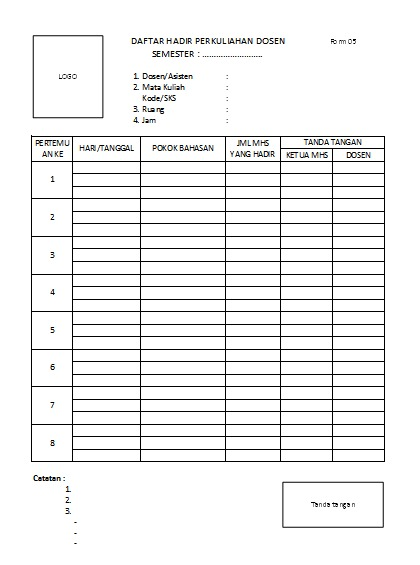
\includegraphics[width=0.7\textwidth]{gambar/form05-gambaran}
	\caption{Form 05}
\end{figure}

\begin{figure}[h!]
	\centering
	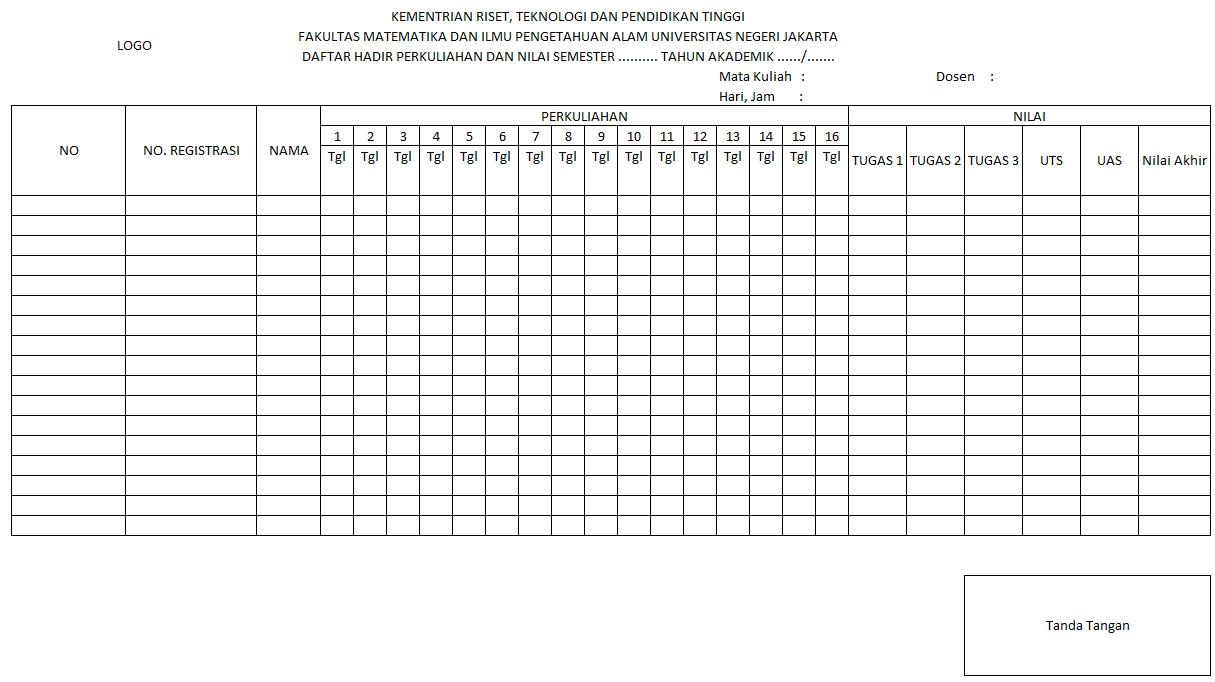
\includegraphics[width=0.7\textwidth]{gambar/form06-gambaran}
	\caption{Form 06}
\end{figure}

	Evaluasi form 05 dan 06 dilakukan tiga kali setiap semester. evaluasi pertama dilakukan pada minggu pertama untuk melihat mulainya pelaksanaan kuliah pertemuan pertama. Evaluasi kedua dilakukan sebelum Ujian Tengah Semester untuk melihat apakah jumlah pertemuan yang dilakukan sesuai atau cukup untuk melaksanakan Ujian Tengah Semester. Evaluasi ketiga dilakukan pada minggu terakhir untuk melihat apakah jumlah pertemuan mencapai syarat minimal 80\%. Evaluasi ini dilakukan oleh Tim Penjamin Mutu program studi dan nantinya akan dilaporkan ke Gugus Penjamin Mutu.


\section{Sistem Informasi}
\subsection{Definisi Sistem}
	Sistem adalah kumpulan atau grup dari bagian atau komponen apapun, baik fisik ataupun non fisik yang saling berhubungan satu sama lain dan bekerja sama untuk mencapai satu tujuan tertentu \citep{Susanto2017}. Sebuah sistem mempunyai karakteristik atau sifat-sifat tertentu, yaitu mempunyai komponen-komponen, batas sistem, lingkungan luar sistem, penghubung, masukan, keluaran, pengolah, dan sasaran atau tujuan \citep{Ladjamudin2005}.

	Menurut \cite{Romney2009}, sistem adalah suatu rangkaian yang terdiri dari beberapa komponen yang saling berhubungan dan saling berinteraksi antara satu sama lain untuk mencapai tujuan. Sistem biasanya terbagi menjadi subsistem yang lebih kecil yang mendukung sistem yang lebih besar. Dari pengertian-pengertian diatas, dapat disimpulkan bahwa sistem adalah kumpulan dari komponen-komponen yang saling berhubungan dan berinteraksi satu sama lain dalam sebuah rangkaian untuk mencapai tujuan.

\subsection{Definisi Informasi}
	Informasi adalah data yang telah diolah ke dalam bentuk yang lebih berguna dan lebih berarti bagi penggunanya. Informasi merupakan salah satu sumber daya paling penting yang dimiliki oleh suatu organisasi. Menurut \cite{Susanto2017} definisi informasi adalah hasil pengolahan data yang memberikan arti dan manfaat. Alat pengolahan informasi dapat berupa komponen komputer, komponen non komputer, atau kombinasi keduanya \citep{Ladjamudin2005}.

	Tidak semua data dapat digunakan untuk mendapatkan informasi yang berkualitas, data tersebut harus memiliki karakteristik tertentu. Untuk mendapat informasi yang berkualitas dibutuhkan data-data yang memiliki karakteristik sebagai berikut \citep{Kroenke2009}:
\begin{enumerate}
	\item Akurat

	Data yang benar, lengkap, dan akurat dan dengan didasarkan pengolahan yang sesuai akan menghasilkan informasi yang berkualitas. Dalam bisnis untuk mengambil keputusan sangatlah membutuhkan data yang akurat. Penggunaan data yang tidak akurat sebagai dasar pengambilan keputusan dapat memberikan dampak yang tidak diinginkan.

	\item Tepat Waktu

	Ketepatan waktu pada suatu informasi memiliki pengaruh yang sangat besar. Maksud dari ketepatan waktu tersebut adalah data yang digunakan dapat tersedia setiap waktu untuk digunakan sesuai kebutuhannya. Mengolah dan menghasilkan data secara cepat dan tepat akan menghasilkan informasi yang berkualitas dan dapat dimanfaatkan dengan tepat.

 Tepat waktu dimaksudkan dengan ketersediaan data setiap waktu diperlukan untuk dapat digunakan untuk kebutuhan tertentu. Infomasi yang berkualitas didapatkan dari data yang dapat diolah dan dihasilkan dengan cepat dan tepat agar pemanfaatannya dapat digunakan dengan tepat. Contohnya, ketika membuat sebuah laporan bulanan pada sebuah instansi, data yang diproses haruslah data yang didapatkan dalam satu bulan dan laporan tersebut harus selesai dengan secepatnya karena akan menjadi pertimbangan manajemen perusahaan dalam membuat keputusan selanjutnya.

	\item Relevan

	Informasi harus didapatkan dari data yang relevan baik dalam konteks maupun subjek. Relevansi data berdasarkan konteks dimaksudkan pada penggunaan data harus sesuai dalam bidangnya. Contohnya, untuk karyawan dengan sistem \textit{payroll}, data jam kerja merupakan data yang relevan dengan pekerjaan karyawan \textit{payroll} tersebut. Namun, daftar data jam kerja tersebut menjadi tidak relevan secara kontekstual jika digunakan untuk karyawan yang tidak menggunakan sistem payroll.

	Relevansi data berdasarkan subjek dimaksudkan pada data yang diatur berdasarkan subjeknya. Contohnya, ketika sebuah instansi membutuhkan data penawaran kredit oleh beberapa bank, maka data suku bunga merupakan data yang relevan berdasarkan subjek bank tersebut.

	\item Cukup

	Data yang cukup juga sangat berpengaruh dengan kualitas informasi yang dihasilkan. Kecukupan data dimaksudkan dengan ketersediaan data yang memenuhi keperluan dan tidak berlebihan dalam mengolah data tersebut menjadi informasi.

	\item Sebanding dengan biaya

	Memperoleh data tidaklah gratis. Ada biaya dalam melakukan pengolahan sebuah data termasuk memelihara sistem pengolah data, membayar gaji karyawan yang mengolah data, dan lain sebagainya. Atas dasar hal tersebut, data harus digunakan dengan bijak sehingga informasi yang dihasilkan dapat mengimbangi biaya yang dikeluarkan dalam mengolah data tersebut menjadi informasi.
\end{enumerate}

\subsection{Definisi Sistem Informasi}
	Sistem informasi adalah sebuah sistem dalam suatu keorganisasian yang mempertemukan kebutuhan pengelolaan, mendukung operasi, bersifat manajerial, dan kegiatan strategi dari suatu organisasi dan menyediakan pihak luar tertentu dengan laporan-laporan yang dibutuhkan \citep{Hutahaean2015}. Sistem informasi merupakan gabungan dari serangkaian komponen yang dapat berupa manusia, prosedur, data, dan teknologi yang digunakan untuk menghasilkan informasi yang bernilai sebagai dasar pengambilan keputusan.

	Sistem informasi memiliki komponen-komponen penting yang berinteraksi satu sama lain dan bekerja sama untuk melakukan suatu proses. Berikut adalah komponen-komponen dalam sistem informasi \citep{Jogiyanto2005}:

\begin{enumerate}

	\item Input, komponen input menjelaskan bagaimana sistem memperoleh atau menyediakan data untuk diproses lebih lanjut.
	\item Process, komponen process menjelaskan bagaimana suatu data diproses sehingga dapat menghasilkan informasi yang lebih bernilai.
	\item Output, komponen output adalah komponen hasil dari proses yang telah dilakukan sebelumnya.
	\item Penyimpanan, komponen penyimpanan merupakan komponen kegiatan yang dilakukan untuk menyimpan dan memelihara data.
	\item Pengendalian, komponen pengendalian merupakan komponen yang menjamin sistem informasi dapat berjalan sesuai yang diharapkan dan merupakan komponen paling penting dalam suatu sistem informasi.
\end{enumerate}
	Berdasarkan teori-teori dan pendapat diatas, dapat disimpulkan bahwa sistem informasi merupakan sebuah sistem dalam suatu organisasi yang bersifat manajerial dengan berbagai komponen yang berinteraksi dan bekerja sama antara satu dengan yang lain yang digunakan untuk menghasilkan informasi yang berkualitas dan dapat menjadi dasar dari suatu pengambilan keputusan.

\section{Software Development Life Cycle (SDLC)}
Proses pengembangan sebuah perangkat lunak dan sistem informasi selalu dipengaruhi oleh beberapa metodologi pengembangan. Metodologi pengembangan perangkat lunak mengacu pada kerangka kerja yang digunakan untuk merencanakan, mengelola, dan mengendalikan proses pengembangan sebuah sistem informasi. Metodologi pengembangan perangkat lunak disebut sebagai siklus hidup pengembangan perangkat lunak atau biasa dikenal sebagai \textit{Software Development Life Cycle}. SDLC adalah proses yang menjelaskan metode dan strategi mendesain dan memelihara proyek perangkat lunak untuk memastikan tujuan, sasaran, fungsional, dan kebutuhan pengguna dapat tercapai \citep{Arora2016}.

Proses pada metodologi SDLC umumnya dibagi menjadi beberapa fase, yaitu \citep{Dora2013}:

\begin{enumerate}
	
	\item \textit{Requirement Analysis}

	\textit{Requrement Analysis} adalah fase pertama dalam SDLC. Tujuan dari \textit{requirement analysis} adalah mengetahui dan mendokumentasikan kebutuhan sebenarnya dari pengguna. Fokus dari \textit{requirement analysis} adalah mengetahui apa yang dibutuhkan dari sistem yang akan dibuat. Fase ini adalah fase paling penting dalam SDLC. Hasil dari \textit{requirement analysis} adalah deskripsi lengkap dan komprehensif dari kegiatan yang dilakukan perangkat lunak yang akan dikembangkan.

	\item \textit{Design}

	Fase desain adalah fase paling kreatif pada SDLC. Pada fase desain, spesifikasi kebutuhan yang ada diubah menjadi bentuk terstruktur atau terencana. Fase ini merupakan proses perencanaan dan \textit{problem solving} untuk mencari solusi dengan perangkat lunak. Hasil dari fase ini adalah dokumen desain dari perangkat lunak yang akan dikembangkan.

	\item \textit{Coding}

	Pada fase \textit{coding}, dokumen desain dari perangkat lunak diubah menjadi \textit{code} dengan menggunakan bahasa pemrogramman tertentu. Fase ini adalah fase \textit{login} dari SDLC. Hasil dari fase ini adalah kode program.

	\item \textit{Testing}

	Segera setelah fase \textit{coding}, \textit{testing} dilakukan untuk mengetahui hasil dari aplikasi yang telah dikembangkan. \textit{Testing} dibuat untuk mengetahui hasil asli dan hasil yang diharapkan. Fase ini adalah fase paling penting dan berpengaruh. \textit{Testing} yang efektif akan menghasilkan produk perangkat lunak dengan kualitas tinggi, akurat, dan hasil yang dapat diandalkan.

	\item \textit{Maintenance}

	Fase akhir dari SDLC, dimana perangkat lunak yang telah dikembangkan didistribusikan ke pengguna akhir untuk pemeliharaan dan menggunakan untuk pengoperasian seharusnya.
\end{enumerate}

	SDLC memiliki berbagai macam model seperti Waterfall, V model, Spiral, Iterative, Agile, Extreme Programming, Scrum, dan lain sebagainya. Model yang akan dipilih dalam penelitian ini adalah Spiral. 

\section{Model Spiral} 

\begin{figure}[H]
	\centering
	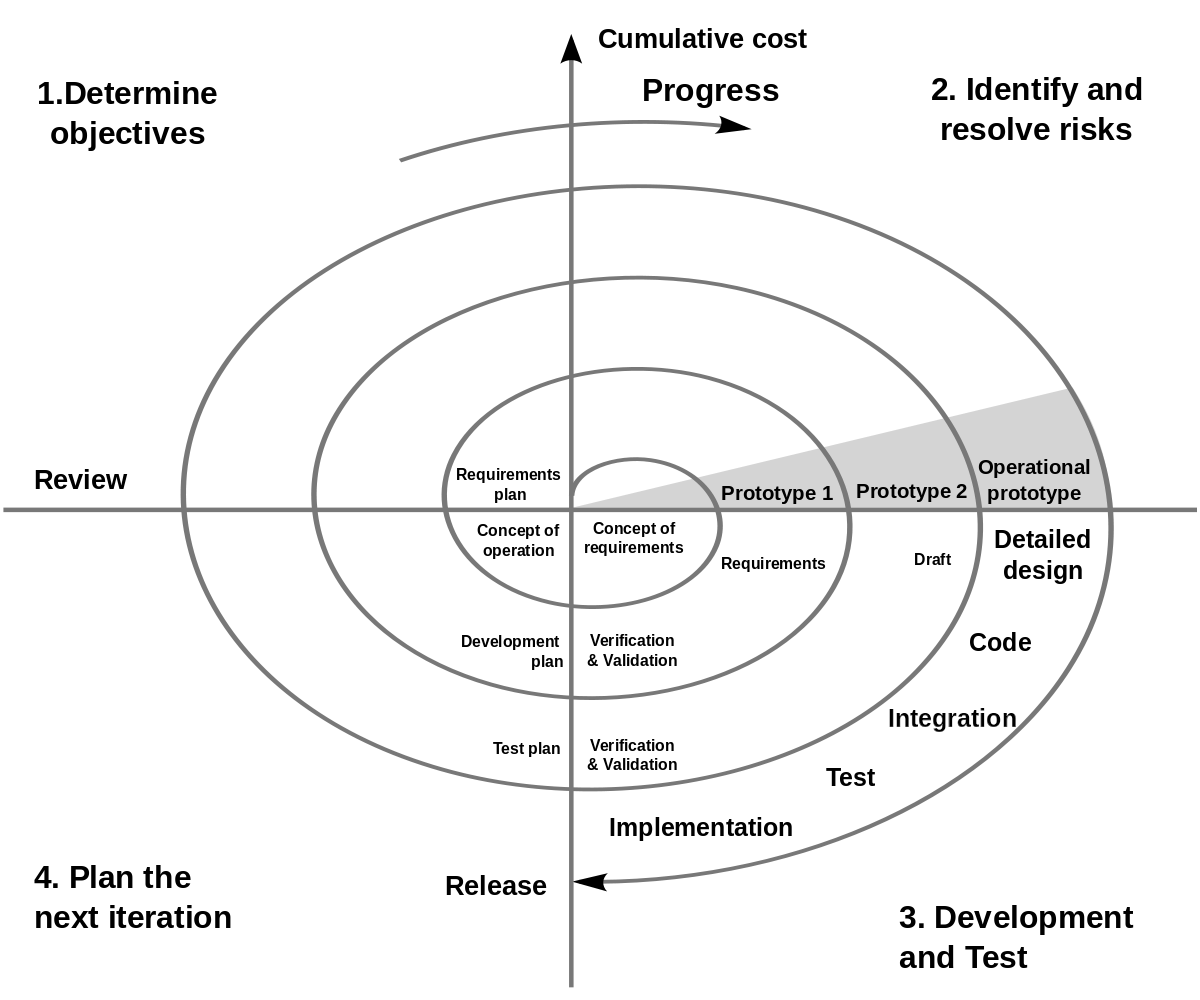
\includegraphics[width=0.7\textwidth]{gambar/Spiral}
	\caption{Model Spiral}
\end{figure}
Model Spiral adalah model SDLC yang menggabungkan proses model Iterative dengan elemen-elemen dari model Waterfall. Model Spiral berfokus pada analisis risiko dan meminimalkan risiko dari proyek. Hal tersebut dilakukan dengan cara membagi sebuah proyek menjadi beberapa bagian kecil sehingga mempermudah jika terdapat perubahan sekaligus melakukan evaluasi risiko dan mempertimbangkan kelanjutan proyek dalam prosesnya. Kemudahan dalam menerapkan model Spiral secara umum ditambah dengan kemudahan dalam melakukan perubahan sistem ketika ada fitur yang ingin ditambahkan ini adalah alasan penulis memilih model Spiral. Tidak seperti model lainnya yang selesai ketika perangkat lunak sudah diberikan ke pengguna, model spiral dapat digunakan sepanjang masa hidup digunakannya perangkat lunak tersebut. Oleh karena itu, iterasi pertama ada spiral dapat berupa konsep proyek yang dimulai pada pusat spiral dan berlanjut untuk beberapa iterasi hingga pengembangan konsep selesai. Jika konsep tersebut akan dibuat menjadi sebuah produk maka proses spiral dilanjutkan dan project pengembangan produk baru dimulai \citep{Pressman2010}. Fase-fase pada model Spiral dapat dideskripsikan sebagai berikut \citep{Alshamrani2015}: 

\begin{enumerate}

	\item Perencanaan

	Fase ini meliputi pemahaman dari kebutuhan sistem dengan melakukan komunikasi yang berkesinambungan antara pengguna dan sistem analis. Pada fase ini ditentukan tujuan yang akan dicapai pada iterasi yang akan berjalan.

	\item Analisis risiko
	
	Dalam fase ini dilakukan sebuah proses untuk mengidentifikasikan risiko yang dapat muncul dan solusi-solusi yang dapat dilakukan. Pada akhir fase ini menghasilkan sebuah prototipe.

	\item Pengembangan

	Pada fase ini program atau perangkat lunak dihasilkan sekaligus dengan dilakukannya pengujian.

	\item Evaluasi

	Fase ini memungkinkan pengguna untuk mengevaluasi hasil dari iterasi proyek sebelum dilanjutkan ke spiral selanjutnya. Pada fase ini dilakukan perencanaan iterasi selanjutnya berdasarkan dengan iterasi yang telah dilakukan.

\end{enumerate}


\section{\textit{Unified Modeling Language} (UML)}
	Menurut Windu dan Grace (2013) dalam jurnal \cite{Suendri2018} \textit{Unified Modeling Language} atau UML adalah bahasa spesifikasi standar yang biasa dipergunakan untuk mendokumentasikan, menspesifikasikan dan membangun perangkat lunak. UML merupakan sebuah metodologi dalam mengembangkan sistem berorientasi objek dan juga merupakan alat untuk mendukung pengembangan sistem.

	Saat ini UML telah menjadi standar bahasa visual yang digunakan untuk memodelkan sistem yang berorientasi objek. Fungsi dari UML adalah untuk melakukan pemodelan sehingga penggunaan dari UML sendiri tidak terbatas pada metodologi tertentu, meskipun pada kenyataannya UML paling banyak digunakan untuk metodologi berorientasi objek.

	Terdapat beberapa jenis diagram UML dan pada penelitian ini akan dibahas beberapa diantarana, yaitu:
\begin{enumerate}

	\item \textit{Use Case Diagram}

	\textit{Use case diagram} adalah diagram UML yang menggambarkan hal-hal apa saja yang dapat dilakukan oleh aktor atau pengguna dalam sistem yang dibuat. Aktor yang dimaksud di dalam \textit{Use Case Diagram} dapat berupa user, sistem internal, atau bahkan sistem eksternal yang dihubungkan dengan sistem yang dibuat. Simbol-simbol yang ada pada use case diagram dapat dilihat pada tabel \ref{tab:usecase}.

\begin{table}[h!]
\centering
\caption{Simbol-Simbol Pada \textit{Use Case Diagram}}
\label{tab:usecase}
\begin{tabular} { |>{\centering\arraybackslash}p{5cm}|p{6cm}| }
	\hline
	\textbf{Simbol} & \multicolumn{1}{>{\centering\arraybackslash}p{6cm}|}{\textbf{Deskripsi}} \\ 
	\hline
	\raisebox{-\totalheight}{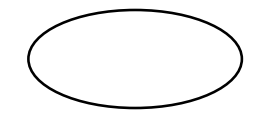
\includegraphics[scale=0.3]{gambar/usecase_usecase}}
	&
		\textit{Use case} adalah langkah atau tindakan yang dapat dilakukan di dalam sistem.
	\\
	\hline
	\raisebox{-\totalheight}{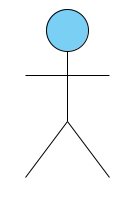
\includegraphics[scale=0.3]{gambar/actor_usecase}}
	&
		Aktor merupakan sebuah abstraksi dari pengguna atau peran yang lain yang terlibat dan berinteraksi dengan sistem.
	\\
	\hline
	\raisebox{-\totalheight}{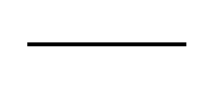
\includegraphics[scale=0.3]{gambar/asosiasi_usecase}}
	&
		Asosiasi adalah hubungan antara aktor dan \textit{use case} yang menggambarkan hubungan interaksi langsung antara keduanya.
	\\
	\hline
	\raisebox{-\totalheight}{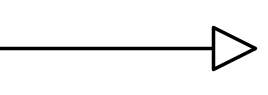
\includegraphics[scale=0.3]{gambar/generalisasi_usecase}}
	&
		Generalisasi adalah hubungan antara aktor yang menggambarkan kesamaan perilaku objek induk dengan objek anak.
	\\
	\hline
	\raisebox{-\totalheight}{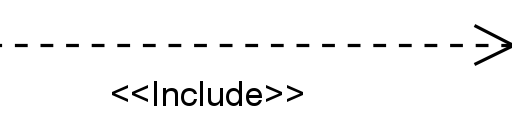
\includegraphics[scale=0.3]{gambar/include_usecase}}
	&
		\textit{Include} adalah hubungan antara \textit{use case} yang menggambarkan kebutuhan suatu \textit{use case} untuk dilanjutkan dengan \textit{use case} lain.
	\\
	\hline
	\raisebox{-\totalheight}{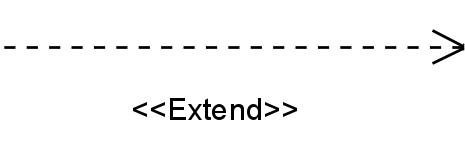
\includegraphics[scale=0.3]{gambar/extend_usecase}}
	&
		\textit{Extend} adalah hubungan antara \textit{use case} yang menggambarkan kemungkinan suatu \textit{use case} untuk dilanjutkan dengan \textit{use case} lain.
	\\
	\hline
\end{tabular}
\end{table}

	\item \textit{Class Diagram}

\textit{Class diagram} adalah sebuah diagram yang digunakan untuk menggambarkan kelas, atribut-atribut kelas, dan hubungan antar setiap kelas. Menurut Whitten dalam jurnal \cite{Suendri2018} kelas adalah suatu set objek yang memiliki atribut dan perilaku yang sama. Hubungan antar kelas dalam \textit{class diagram} memiliki keterangan yang biasa disebut dengan \textit{Multiplicity} atau \textit{Cardinality}. Ada beberapa jenis \textit{Multiplicity} sebagaimana digambarkan pada tabel \ref{tab:multiplicitybab2}. Simbol-simbol yang ada pada \textit{class diagram} dapat dilihat pada tabel \ref{tab:classdiagram}.

\begin{table}[h!]
\centering
\caption{\textit{Multiplicity} atau \textit{Cardinality} pada \textit{Class Diagram}}
\label{tab:multiplicitybab2}
\begin{tabular} { |>{\centering\arraybackslash}p{4cm}|p{5cm}| }
	\hline
	\textbf{\textit{Multiplicity}} & \multicolumn{1}{>{\centering\arraybackslash}p{6cm}|}{\textbf{Deskripsi Hubungan}} \\ 
	\hline

	1
	&
		Satu dan hanya satu.
	\\
	\hline
	0..*
	&
		Boleh tidak ada atau ada.
	\\
	\hline
	0..1
	&
		Boleh tidak ada atau hanya satu.
	\\
	\hline
	1..*
	&
		Harus ada dan boleh lebih dari satu.
	\\
	\hline
	n..m
	&
		Batasan jarak antara n dan m. Minimal n dan maksimal m.
	\\
	\hline
\end{tabular}
\end{table}

\begin{table}[h!]
\centering
\caption{Simbol-Simbol Pada \textit{Class Diagram}}
\label{tab:classdiagram}
\begin{tabular} { |>{\centering\arraybackslash}p{5cm}|p{6cm}| }
	\hline
	\textbf{Simbol} & \multicolumn{1}{>{\centering\arraybackslash}p{6cm}|}{\textbf{Deskripsi}} \\
	\hline
	\raisebox{-\totalheight}{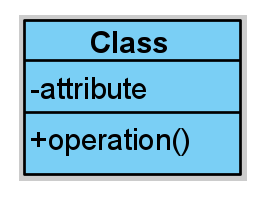
\includegraphics[scale=0.3]{gambar/classdiagram_kelas}}
	&
		Kelas merupakan elemen dan interaksi utama pada aplikasi.
	\\
	\hline
	\raisebox{-\totalheight}{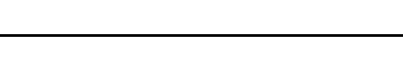
\includegraphics[scale=0.3]{gambar/classdiagram_asosiasi}}
	&
		Asosiasi adalah hubungan atau relasi umum antara kelas yang disertai dengan \textit{multiplicity}.
	\\
	\hline
	\raisebox{-\totalheight}{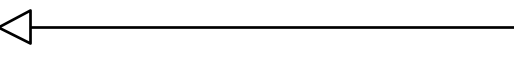
\includegraphics[scale=0.3]{gambar/classdiagram_generalisasi}}
	&
		Generalisasi adalah hubungan antara kelas yang menjelaskan bahwa suatu kelas merupakan \textit{superclass} dari kelas yang lain.
	\\
	\hline
	\raisebox{-\totalheight}{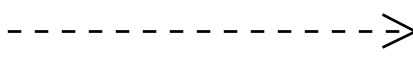
\includegraphics[scale=0.3]{gambar/classdiagram_depedensi}}
	&
		Generalisasi adalah hubungan antara kelas yang menggambarkan kesamaan perilaku \emph{superclass} dan \emph{subclass}
	\\
	\hline
	\raisebox{-\totalheight}{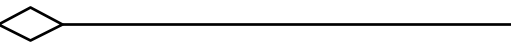
\includegraphics[scale=0.3]{gambar/classdiagram_agregat}}
	&
		Agregasi adalah hubungan atau relasi antar kelas yang bermakna semua objek kelas merupakan bagian dari kelas lain.
	\\
	\hline
	
\end{tabular}
\end{table}

	\item \textit{Activity Diagram}

	\textit{Activity diagram} adalah diagram yang digunakan untuk menggambarkan proses jalannya suatu aktivitas atau kegiatan yang dapat dilakukan dalam sebuah sistem. \textit{Activity diagram} biasanya menggambarkan bagaimana masing-masing kegiatan dimulai, keputusan yang mungkin terjadi di dalam kegiatan tersebut, hingga berakhirnya kegiatan yang dilakukan. \textit{Activity diagram} dapat menggambarkan lebih dari satu proses aksi dalam waktu bersamaan. Menurut Haviluddin dalam jurnal \cite{Suendri2018} \textit{Activity diagram} adalah aktivitas-aktivitas, objek, \textit{state}, transisi \textit{state}, dan \textit{event}. Dengan kata lain kegiatan diagram alur kerja menggambarkan perilaku sistem untuk aktivitas. Simbol-simbol yang digunakan pada activity diagram dapat dilihat pada tabel \ref{tab:activitydiagram}.

\begin{table}[h!]
\centering
\caption{Simbol-Simbol Pada \textit{Activity Diagram}}
\label{tab:activitydiagram}
\begin{tabular} { |>{\centering\arraybackslash}p{5cm}|p{6cm}| }
	\hline
	\textbf{Simbol} & \multicolumn{1}{>{\centering\arraybackslash}p{6cm}|}{\textbf{Deskripsi}} \\ 
	\hline
	\raisebox{-\totalheight}{
\includegraphics[scale=0.3]{gambar/activitydiagram_startpoint}}
	&
		\textit{Start Point} adalah poin dimulainya \textit{activity}.
	\\
	\hline
	\raisebox{-\totalheight}{
\includegraphics[scale=0.3]{gambar/activitydiagram_endpoint}}
	&
		\textit{End Point} adalah poin berakhirnya \textit{activity}.
	\\
	\hline
	\raisebox{-\totalheight}{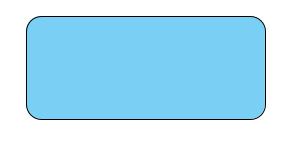
\includegraphics[scale=0.3]{gambar/activitydiagram_activity}}
	&
		\textit{Activity} menggambarkan suatu kegiatan atau proses bisnis.
	\\
	\hline
	\raisebox{-\totalheight}{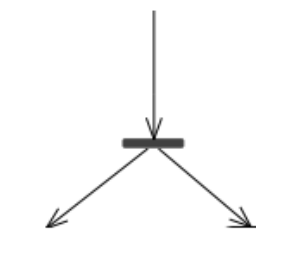
\includegraphics[scale=0.3]{gambar/activitydiagram_fork}}
	&
		\textit{Fork} adalah pembagian sebuah kegiatan menjadi lebih dari satu.
	\\
	\hline
	\raisebox{-\totalheight}{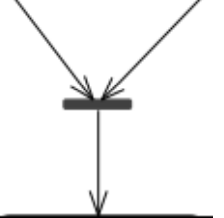
\includegraphics[scale=0.3]{gambar/activitydiagram_join}}
	&
		\textit{Join} adalah penggabungan kegiatan menjadi satu.
	\\
	\hline
	\raisebox{-\totalheight}{
\includegraphics[scale=0.3]{gambar/activitydiagram_decisionnode}}
	&
		\textit{Decision Node} adalah pembagian sebuah kegiatan menjadi lebih dari satu berdasarkan keputusan yang diambil.
	\\
	\hline
	
\end{tabular}
\end{table}

\begin{comment}
	\item Sequence Diagram

	Sequence Diagram adalah salah satu tipe diagram interaksi yang menggambarkan bagaimana sekumpulan objek bekerja sama dan dalam urutan yang bagaimana. Menurut Haviluddin dalam jurnal \cite{Suendri2018} secara mudahnya sequence diagram adalah gambaran tahap demi tahap, termasuk kronologi (urutan) perubahan secara logis yang seharusnya dilakukan untuk menghasilkan sesuatu sesuai dengan use case diagram. Beberapa simbol-simbol yang digunakan dalam sequence diagram dapat dilihat pada tabel 

\begin{table}[h!]
\centering
\caption{Simbol-Simbol Pada Sequence Diagram}
\label{tab:sequencediagram}
\begin{tabular} { |>{\centering\arraybackslash}p{5cm}|p{6cm}| }
	\hline
	\textbf{Simbol} & \multicolumn{1}{>{\centering\arraybackslash}p{6cm}|}{\textbf{Deskripsi}} \\ 
	\hline
	\raisebox{-\totalheight}{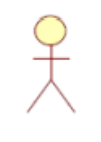
\includegraphics[scale=0.5]{gambar/sequencediagram_actor}}
	&
		Actor adalah sebuah abstraksi dari pengguna atau peran yang lain yang terlibat dan berinteraksi dengan sistem.
	\\
	\hline
	\raisebox{-\totalheight}{
\includegraphics[scale=0.5]{gambar/sequencediagram_entityclass}}
	&
		Entity class adalah kelas yang berupa entitas-entitas utama sistem. Entity menggambarkan data pada sistem.
	\\
	\hline
	\raisebox{-\totalheight}{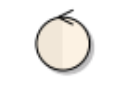
\includegraphics[scale=0.5]{gambar/sequencediagram_controlclass}}
	&
		Control class adalah kelas yang berisi logika-logika yang mengatur elemen-elemen pada sistem dan interaksinya.
	\\
	\hline
	\raisebox{-\totalheight}{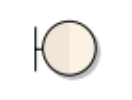
\includegraphics[scale=0.5]{gambar/sequencediagram_boundaryclass}}
	&
		Boundary class adalah kelas yang digunakan untuk memodelkan interaksi antara aktor dalam sistem.
	\\
	\hline
	\raisebox{-\totalheight}{
\includegraphics[scale=0.3]{gambar/sequencediagram_message}}
	&
		Message adalah pesan yang dikirimkan antara class.
	\\
	\hline
	\raisebox{-\totalheight}{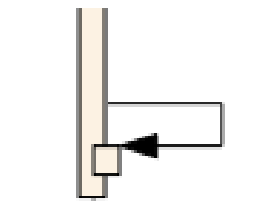
\includegraphics[scale=0.3]{gambar/sequencediagram_recursive}}
	&
		Recursive adalah pesan yang dikirimkan untuk class itu sendiri.
	\\
	\hline
	\raisebox{-\totalheight}{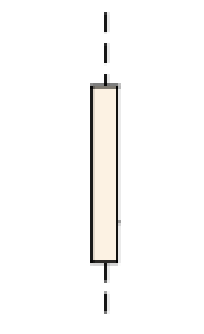
\includegraphics[scale=0.3]{gambar/sequencediagram_activation}}
	&
		Activation menggambarkan sebuah eksekusi operasi pada objek tersebut.
	\\
	\hline
	
\end{tabular}
\end{table}
\end{comment}

\end{enumerate}

\section{\textit{Entity Relationship Diagram}}

	\emph{Entity Relationship Diagram} (ERD) adalah sebuah tipe diagram struktural yang digunakan untuk mendesain \textit{database}. ERD memiliki banyak simbol dan penghubung yang digunakan untuk menggambarkan dua informasi penting, yaitu entitas utama dalam lingkup sistem dan hubungan antara masing-masing entitas yang ada. Menurut Simarmata(2010:67) dalam jurnal \cite{Fridayanthie2016} ERD adalah alat pemodelan data utama dan akan membantu mengorganisasi data dalam suatu proyek ke dalam entitas-entitas dan menentukan hubungan antar entitas. Sebuah ERD terdiri dari tiga komponen utama yaitu:

\begin{enumerate}

	\item \textit{Entity}

	\textit{Entity} atau entitas adalah sebuah benda atau konsep yang dapat didefinisikan di dalam sistem seperti Mahasiswa, Profil, Nilai, dan lain-lain. Notasi entitas biasanya dilambangkan dengan persegi panjang dengan nama dari entitas tersebut di atasnya dan berisi atribut dari entitas tersebut 

	\item \textit{Attribute}

	\textit{Attribute} adalah properti atau karakteristik dari suatu entitas. Sebuah atribut memiliki nama yang menjelaskan karakteristiknya dan tipe yang menjelaskan jenis dari karakteristik tersebut seperti \textit{varchar} atau \textit{int}. Sebagai contoh dalam entitas Mahasiswa terdapat atribut nama, nomor registrasi, alamat, dan lain-lain.

	\item \textit{Relationship}

	\textit{Relationship} dalam ERD adalah hubungan antara dua entitas yang menggambarkan bahwa kedua entitas tersebut memiliki suatu kaitan tertentu. Sebagai contoh seorang mahasiswa dapat mendaftarkan kelas yang ingin diikuti. \textit{Relationship} didefinisikan dengan menggunakan \textit{Foreign} \textit{Key} yang mengacu pada sebuah \textit{Primary Key}.
\end{enumerate}


\begin{figure}[H]
	\centering
	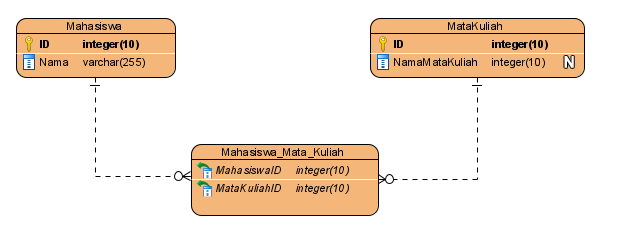
\includegraphics[width=1\textwidth]{gambar/contoh_erd}
	\caption{Contoh Sederhana ERD}
\end{figure}

\section{\textit{Database}}

	\textit{Database} merupakan sebuah kumpulan data-data yang terstruktur sehingga menjadi suatu informasi yang dapat dimanfaatkan. \textit{Database} terbentuk dari sekelompok data-data yang memiliki jenis atau sifat yang sama. Contohnya \textit{database} karyawan dapat berisi data-data berupa nama-nama, divisi-divisi, dan jabatan-jabatan karyawan.


	\textit{Database} adalah komponen yang paling penting dalam pembangunan sebuah sistem informasi, karena \textit{database} merupakan tempat untuk menyimpan dan mengelola seluruh data yang dimiliki. Data diatur sedemikian rupa sehingga tidak ada data yang terduplikasi agar data dapat diolah dengan tepat dan mudah untuk menghasilkan informasi.

	Menurut Susanto dalam jurnal \cite{Sudrajat2014} \textit{database} atau basis data adalah suatu kumpulan data terhubung (\textit{interrelated data}) yang disimpan secara bersama-sama dalam suatu media, tanpa mengatap satu sama lain atau tidak perlu kerangkapan data, data disimpan dengan cara-cara tertentu sehingga mudah untuk digunakan atau ditampilkan kembali. \textit{Database} dapat didefinisikan sebagai kumpulan data yang terintegrasi dan diatur sedemikian rupa sehingga data tersebut dapat dimanipulasi, diambil, dan dicari secara cepat \citep{Raharjo2011}.

	Untuk mengelola sebuah \textit{database} diperlukan sebuah perangkat lunak khusus yang disebut \textit{Database Management System} atau biasa disebut DBMS. DBMS adalah sebuah program yang digunakan untuk membuat, mendefinisikan, dan memelihara database. DBMS yang akan digunakan dan dibahas pada penelitian ini adalah MySQL yang juga merupakan salah satu DBMS yang paling banyak digunakan. MySQL merupakan sebuah DBMS \textit{Open Source} sehingga \textit{source code} dari MySQL dapat diakses secara umum dan dapat diunduh secara gratis. Menurut MySQL \textit{manual}, MySQL merupakan  perangkat lunak \textit{database} berbasis SQL (\textit{Structured Query Language}) yang dapat menangani sistem manajemen \textit{database} dan sistem manajemen \textit{database} relasional.

	Sebagai sebuah DBMS, MySQL memiliki beberapa fitur seperti:

\begin{enumerate}

	\item \textit{Multiplatform}

	MySQL tersedia pada berbagai platform umum seperti Windows, Linux, Unix, dan lain-lain.

	\item Dukungan SQL

	SQL sudah menjadi standar pada penggunaan \textit{database} relasional. Memiliki pengetahuan SQL akan sangat memudahkan penggunaan MySQL.

	\item Jaminan keamanan akses

	MySQL memberikan jaminan keamanan \textit{database} dengan beberapa kriteria pengaksesan.

	\item Cepat, handal, dan mudah digunakan

	MySQL termasuk sebagai \textit{database} \textit{server} yang handal, dapat menangani \textit{database} dengan ukuran besar dengan cepat, memiliki banyak fungsi pengaksesan, dan juga mudah digunakan.
\end{enumerate}

\section{\textit{Web Service}}

	\textit{Service} dalam dunia komputer adalah sebuah fungsionalitas dari program perangkat lunak yang dibuat untuk melayani kebutuhan dari program lain. Sebuah \textit{service} bertujuan untuk memungkinkan beberapa program lainnya untuk menggunakan \textit{service} tersebut dengan berbagai macam tujuan.  Menurut Wahli dkk dalam jurnal \cite{Fauziah2013} \textit{web sevice} merupakan suatu aplikasi modular yang bersifat mandiri dan dapat dipublikasikan, dialokasikan dan dipanggil melalui sebuah jaringan. Tujuan dari dibuatnya \textit{web service} adalah untuk membuat sebuah fungsionalitas yang dapat diakses melalui \textit{Internet Protocol} (IP) yang tidak bergantung pada platform dan bahasa pemrograman yang digunakan. \textit{Web service} dapat menjalankan fungsionalitas bisnis mulai dari yang sederhana seperti \textit{request-reply} hingga interaksi bisnis proses sepenuhnya. Untuk menjalankan proses yang rumit, sebuah \textit{web service} dapat bekerja sama atau mengandalkan \textit{web service} lain.

	\textit{Web service} dapat dibangun menggunakan beberapa bentuk arsitektur, salah satunya yang akan dibahas adalah \textit{Representational State Transfer}(REST). \textit{Web service} yang dibuat mengikuti arsitektur REST disebut RESTful \textit{Web Service}. Pada RESTful \textit{web} \textit{service}, \textit{server} menyediakan data atau sumber daya dan \textit{client} dapat mengakses data tersebut untuk digunakan. Setiap data atau \textit{resource} pada REST \textit{server} diidentifikasi oleh \textit{global id} yang merupakan URIs (\textit{Universal Resource Identifiers}). Pada umumnya data tersebut diberikan dalam format teks seperti JSON atau XML.

	Metode-metode HTTP yang biasa digunakan dalam RESTful \textit{Web Service} adalah sebagai berikut:

\begin{enumerate}

	\item \textit{Get}

		\textit{Get} adalah metode untuk membaca data.

	\item \textit{Post}

		\textit{Post} adalah metode untuk membuat data baru.

	\item \textit{Delete}

		\textit{Delete} adalah metode untuk menghapus data.

	\item \textit{Put}
		\textit{Put} adalah metode untuk memperbarui data yang sudah ada atau membuat data baru jika data belum ada.
\end{enumerate}

\section{\textit{Framework}}

	\textit{Framework} atau kerangka kerja adalah desain keseluruhan atau sebagian dari sistem yang berupa sebuah kumpulan kelas abstrak dan fungsi-fungsinya yang digunakan untuk mempermudah pengembangan sebuah perangkat lunak. Dengan menggunakan sebuah \textit{framework}, seorang \textit{developer} tidak perlu lagi mengimplementasikan fungsi-fungsi umum yang biasa digunakan karena sudah disediakan oleh \textit{framework} yang digunakan sehingga \textit{developer} hanya perlu menyesuaikan dengan kebutuhan dari program yang akan dibuat. \textit{Framework} dalam pembuatan \textit{website} umumnya terdapat dua jenis, yaitu \textit{framework} untuk membuat tampilan pengguna atau \textit{frontend} dan \textit{framework} untuk membuat sisi \textit{server} atau \textit{backend}. Beberapa \textit{framework} juga dapat digunakan untuk membangun keseluruhan dari sebuah \textit{website} mulai dari \textit{frontend} hingga \textit{backend}. Beberapa \textit{framework} yang dapat digunakan untuk membuat \textit{frontend} adalah AngularJS, ReactJS, dan VueJS. Sedangkan untuk \textit{backend} dapat menggunakan CI, Laravel, dan ExpressJS. Pada penelitian ini, digunakan dua \textit{framework} untuk membuat \textit{frontend} dan \textit{backend}, yaitu VueJS dan Laravel.

\section{MVC}

		Konsep MVC adalah sebuah pola desain perangkat lunak yang biasa digunakan untuk membangun user interface yang memisahkan logika pada program yang dibuat menjadi tiga elemen yang saling berhubungan. Tiga elemen tersebut adalah:

\begin{enumerate}

	\item \textit{Model}

	\textit{Model} merupakan komponen yang digunakan untuk mendefinisikan data-data utama yang akan digunakan dan berhubungan langsung dengan \textit{database}. \textit{Model} berisi struktur dari data yang akan digunakan beserta fungsi-fungsi yang bertujuan untuk mengolah data tersebut.

	\item \textit{View}

	\textit{View} adalah komponen yang mengatur tampilan \textit{website} yang dilihat oleh pengguna. Pada komponen inilah bagan, tabel, dan berbagai bentuk tampilan diproses. Umumnya komponen \textit{view} berupa \textit{file} HTML. Pada Laravel komponen \textit{view} bisa menggunakan \textit{templating} \textit{engine} Blade atau bisa menggunakan \textit{framework} Vue.JS.

	\item \textit{Controller}

	\textit{Controller} adalah komponen yang berisi segala logika dan alur kerja dari sistem. \textit{Controller} mengubah input yang diterima dari pengguna dan menentukan perintah selanjutnya yang akan dilaksanakan oleh aplikasi.

\end{enumerate}

		
\begin{figure}[h!]
	\centering
	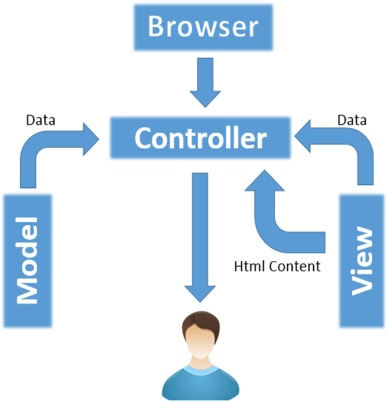
\includegraphics[width=0.5\textwidth]{gambar/mvc}
	\caption{Pola Desain MVC}
\end{figure}


	Selain dari memisahkan aplikasi menjadi tiga, konsep MVC juga mendefinisikan interaksi antara ketiganya. Ketika pengguna menggunakan aplikasi website, pengguna tersebut sedang berinteraksi dengan komponen view. Komponen view lalu menerima input dari pengguna dan meneruskan input tersebut ke controller. Controller lalu mengambil atau mengubah data pada model. Setelah mendapat data yang dibutuhkan Controller lalu mengembalikan data tersebut dan memperbarui view.




% Baris ini digunakan untuk membantu dalam melakukan sitasi
% Karena diapit dengan comment, maka baris ini akan diabaikan
% oleh compiler LaTeX.
\begin{comment}
bibliography{daftar-pustaka}
\end{comment}


%!TEX root = ./template-skripsi.tex
%-------------------------------------------------------------------------------
%                            BAB III
%               			PEMBAHASAN
%-------------------------------------------------------------------------------

\chapter{IMPLEMENTASI PROGRAM}


\section{Analisis Kebutuhan }
Pada tahapan ini, penulis mengumpulkan informasi tentang kebutuhan dari perangkat lunak yang akan dikembangkan dengan cara mewawancara beberapa pihak seperti Koordinator Program Studi, Tim Penjamin Mutu Prodi, dan Gugus Penjamin Mutu FMIPA yang dapat dilihat pada Lampiran A. Penulis juga mengumpulkan informasi dari pengumpulan data pada penelitian serupa yang sebelumnya pernah dilakukan yaitu penelitian yang dilakukan oleh \cite{FitriAndiniMedIrzal2017} yang berjudul "Perancangan dan Implementasi Sistem Absensi Online Berbasis Android di Linkungan Universitas Negeri Jakarta"  dan \cite{Kultsum2021} yang berjudul ''Rancang Bangun Sistem Presensi Akademik Berbasis Web Dengan \textit{Framework} Laravel di Lingkungan Program Studi Ilmu Komputer Universitas Negeri Jakarta''. Berikut beberapa hasil kebutuhan yang penulis dapatkan:

\begin{enumerate}
	\item Sistem memiliki lima jenis pengguna yaitu mahasiswa, penanggung jawab mata kuliah, dosen, tim penjamin mutu, dan admin.
	\item Mahasiswa dapat melihat kelas-kelas yang diambil, mengisi presensi ketika sudah ada pertemuan atau form 05 yang diisi oleh penanggung jawab atau dosen, dan melihat nilai tugas-tugas yang telah diisi oleh dosen.
	\item Penanggung jawab mata kuliah adalah bagian dari mahasiswa dengan tugas tambahan yaitu  mengisi atau memvalidasi form 05. Penanggung jawab mata kuliah dipilih oleh dosen pada pertemuan pertama.
	\item Dosen dapat melihat kelas-kelas yang diampu, mengisi form 05 untuk pertemuan pada kelas tersebut, dan dapat menutup waktu presensi untuk mahasiswa. Untuk memvalidasi presensi dari mahasiswa Dosen dapat memilih untuk memvalidasi semua presensi yang masuk, melakukan seleksi validasi presensi yang sudah masuk, atau memvalidasi semua presensi yang masuk sebelum waktu yang ditentukan.  Dosen juga dapat menambahkan tugas dan mengisi nilai tugas setiap mahasiswa dengan mengunduh format excel yang telah tersedia dan mengunggah \textit{file excel} tersebut ketika ada pembaruan. Ketika penanggung jawab mata kuliah tidak bisa hadir, dosen juga dapat menunjuk penanggung jawab mata kuliah sementara untuk pertemuan tersebut.
	\item Tim penjamin mutu adalah bagian dari dosen dengan tambahan yaitu memiliki menu monitoring yang berisi informasi semua kelas-kelas pada program studi termasuk yang tidak diampu oleh dosen tersebut. Tim penjamin mutu hanya dapat melihat form 05 dan form 06 tanpa bisa merubah data di dalamnya.
	\item Admin hanya memiliki satu tugas yaitu untuk mengatur atau mengubah jenis user dosen atau tim penjamin mutu jika ada perubahan.
	\item Satu kelas bisa diampu lebih dari satu dosen.
	
\end{enumerate}


\section{Implementasi Spiral}


Pada penelitian ini, penulis mengembangkan perangkat lunak dengan menggunakan proses model Spiral dimana pengembangan dilakukan dalam \emph{cycle} atau iterasi. Dari hasil analisis kebutuhan yang telah dilakukan, penulis mengambil beberapa diantaranya untuk dikembangkan dalam iterasi pertama. Total iterasi yang direncanakan adalah tiga iterasi dengan periode waktu satu hingga dua minggu per iterasi. Berikut adalah fase-fase yang penulis jalankan dalam iterasi pertama.

\section{Perencanaan}

Dalam tahap perencanaan, penulis membuat desain-desain dari beberapa kebutuhan yang telah didapatkan dalam bentuk \textit{Use Case Diagram}, \textit{Activity Diagram}, dan rancangan tampilan antarmuka untuk menjadi tujuan yang akan dikembangkan dalam iterasi yang dijalankan. Selain itu, dalam iterasi pertama penulis juga membuat desain rancangan sistem secara keseluruhan dalam bentuk \textit{Entity Relation Diagram}. Iterasi ini berjalan selama dua minggu.

%gambar use case
\subsection{Use Case Diagram}

Pada iterasi pertama, penulis mengembangkan sistem dari sisi mahasiswa terlebih dahulu dikarenakan penulis dapat mengakses \textit{web service} SIAKAD dengan akun mahasiswa penulis. Berikut adalah use case diagram yang telah dibuat:

\begin{figure}[H]
	\centering
	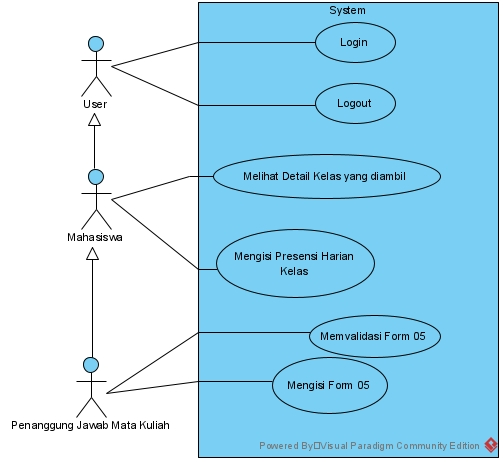
\includegraphics[width=0.8\textwidth]{gambar/diagram/Use Case Iteration 1}
	\caption{Desain \textit{Use Case Diagram Iterasi Pertama}}
	\label{fig:usecase1st}
\end{figure}

Aktor Mahasiswa dapat melihat detail kelas-kelas yang diambil seperti presensi dan nilai setiap mahasiswa pada kelas tersebut dan mengisi presensi pertemuan yang sedang berlangsung.
Aktor Penanggung Jawab Mata Kuliah dapat digeneralisasi menjadi aktor Mahasiswa sehingga mendapat wewenang yang sama seperti aktor Mahasiswa. Aktor penanggung jawab mata kuliah juga dapat mengisi form 05 atau memvalidasi form 05 yang telah dibuat oleh dosen dan memvalidasi presensi form 06 mahasiswa lain.

\subsection{Activity Diagram}

Dari beberapa \textit{use case} yang telah dibuat, penulis juga membuat \textit{activity diagram} untuk beberapa \textit{use case} yang butuh penjelasan alur untuk menjalankannya. Berikut adalah \textit{activity diagram} yang telah dibuat:

\begin{figure}[h!]
	\centering
	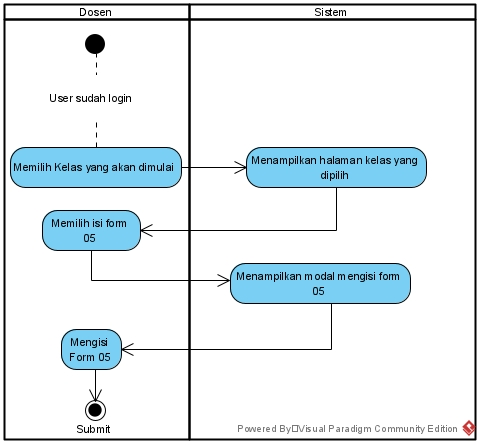
\includegraphics[width=0.7\textwidth]{gambar/diagram/Mengisi Form 05}
	\caption{\textit{Activity} Mengisi Form 05}
	\label{fig:activity2}
\end{figure}

\begin{figure}[h!]
	\centering
	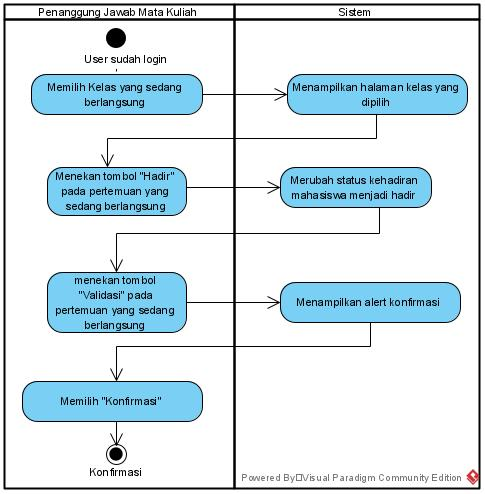
\includegraphics[width=0.7\textwidth]{gambar/diagram/Mengisi Presensi dan Memvalidasi Form 05}
	\caption{\textit{Activity} Mengisi Presensi dan Memvalidasi Form 05}
	\label{fig:activity1}
\end{figure}

Pada gambar \ref{fig:activity2} menggambarkan aktivitas mengisi form 05 yang dapat dilakukan oleh penanggung jawab mata kuliah dan dosen. Pada pengisiannya, penanggung jawab mata kuliah dapat mengosongkan terlebih dahulu materi pembelajaran untuk nantinya ditambahkan oleh dosen.
Pada gambar \ref{fig:activity1} menggambarkan aktivitas mengisi presensi yang dapat dilakukan oleh setiap mahasiswa dan memvalidasi form 05 yang dapat dilakukan oleh penanggung jawab dan dosen.

\subsection{Rancangan Tampilan Antarmuka}

Pada rancangan tampilan antar muka program, penulis membuat desain awal dengan menggunakan \textit{tools online}. Pada halaman \textit{login} yang dapat dilihat pada gambar \ref{fig:login}, user mengisi email dan \textit{password} yang terdaftar pada \textit{web service} SIAKAD.

\begin{figure}[h!]
	\centering
	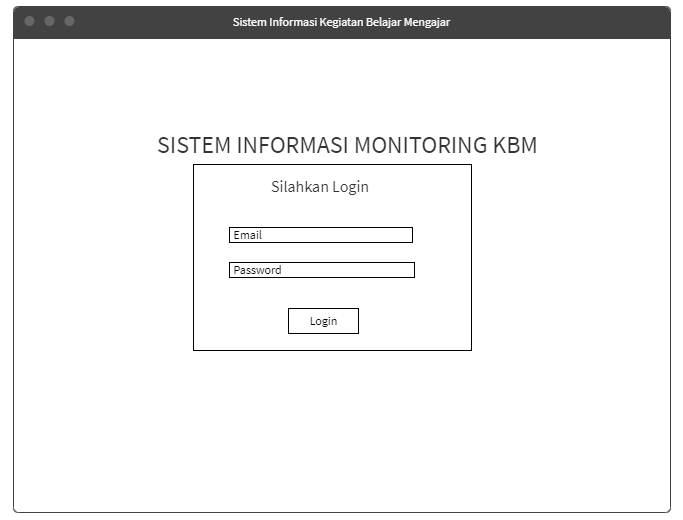
\includegraphics[width=0.8\textwidth]{gambar/mockup/login}
	\caption{Desain Halaman \textit{Login}}
	\label{fig:login}
\end{figure}

Setelah \textit{user} berhasil melakukan \textit{login}, \textit{user} akan dibawa ke halaman \textit{dashboard} dengan menu yang sedikit berbeda bagi setiap jenis \textit{user}. Pada \textit{user} mahasiswa yang dapat dilihat pada gambar \ref{fig:dashboard}, menu yang akan ditampilkan adalah \textit{Home}, Rekap Presensi, dan daftar kelas yang diambil oleh mahasiswa tersebut.

\begin{figure}[h!]
	\centering
	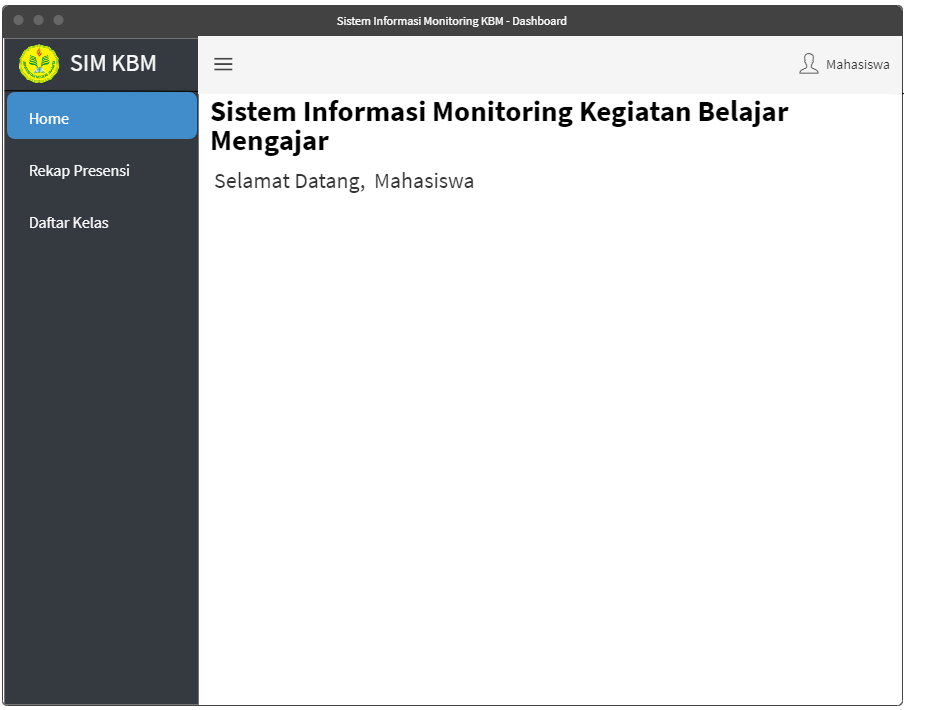
\includegraphics[width=0.8\textwidth]{gambar/mockup/home_mahasiswa}
	\caption{Desain Halaman \textit{Dashboard} Pada mahasiswa}
	\label{fig:dashboard}
\end{figure}


Menu Daftar Kelas merupakan menu yang digunakan untuk membuka halaman kelas yang diambil. Halaman Daftar Kelas dapat dilihat pada gambar \ref{fig:daftarkelas}. Menu kelas terdapat empat bagian \textit{tab} di dalamnya, yaitu Pertemuan, Presensi, Tugas, dan Nilai. Pada \textit{tab} pertemuan yang dapat dilihat pada gambar \ref{fig:form05dosen} dosen dapat menambah pertemuan, memvalidasi form yang dibuat oleh penanggung jawab, memvalidasi presensi mahasiswa, dan mengisi pokok bahasan yang dibahas pada pertemuan tersebut. Setelah pertemuan sudah dibuat dan mahasiswa sudah mengisi presensi, dosen juga bisa memvalidasi presensi mahasiswa tersebut. Pada \textit{tab} ini mahasiswa dapat memilih Hadir untuk mengisi presensi pada pertemuan tersebut yang bisa dilihat pada gambar \ref{fig:form05mhs}. Penanggung jawab mata kuliah memiliki fungsi yang sama dengan mahasiswa dan dosen.

\begin{figure}[h!]
	\centering
	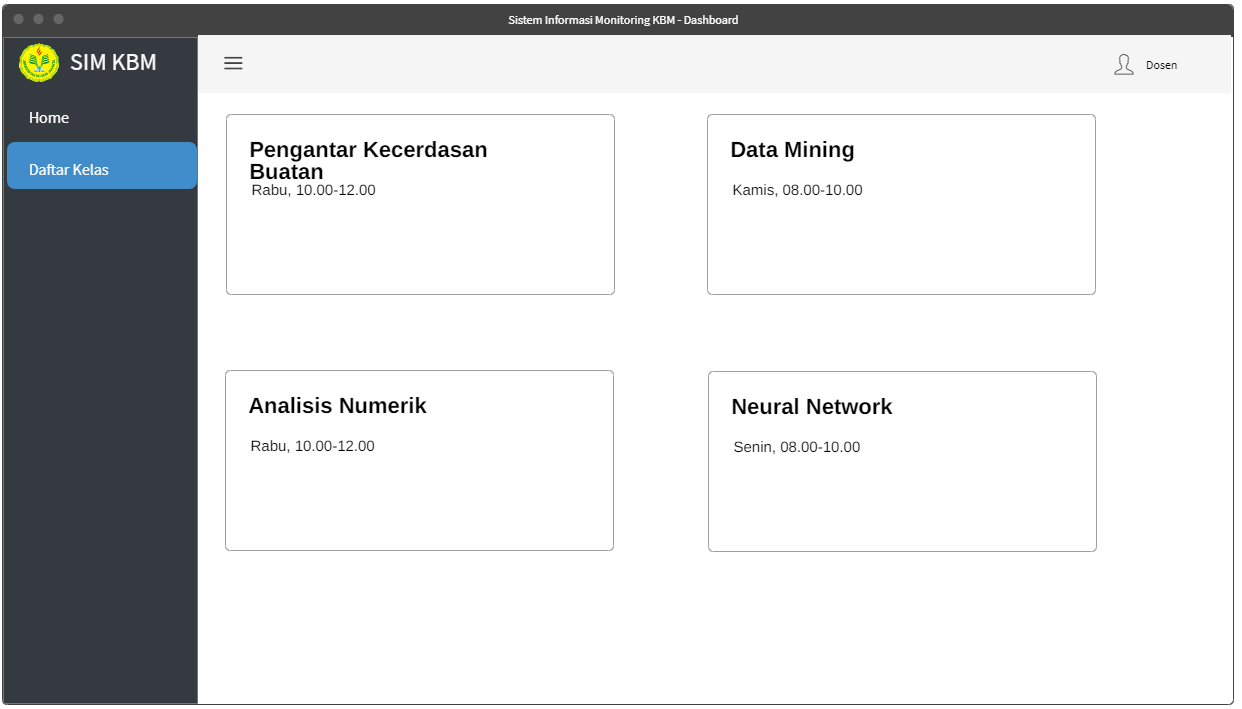
\includegraphics[width=0.8\textwidth]{gambar/mockup/daftar_kelas}
	\caption{Desain Halaman Daftar Kelas}
	\label{fig:daftarkelas}
\end{figure}

\begin{figure}[h!]
	\centering
	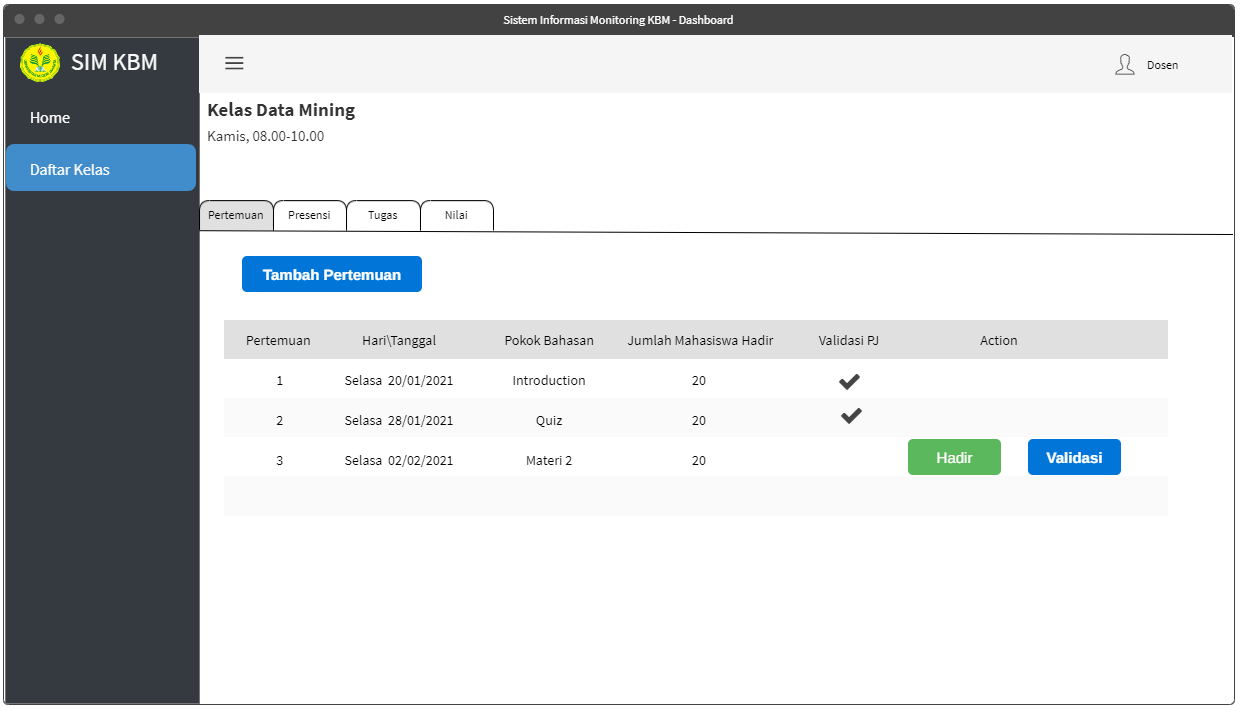
\includegraphics[width=0.8\textwidth]{gambar/mockup/form05_pj}
	\caption{Desain Halaman Form 05 Pada Penanggung Jawab}
	\label{fig:form05pj}
\end{figure}

\begin{figure}[h!]
	\centering
	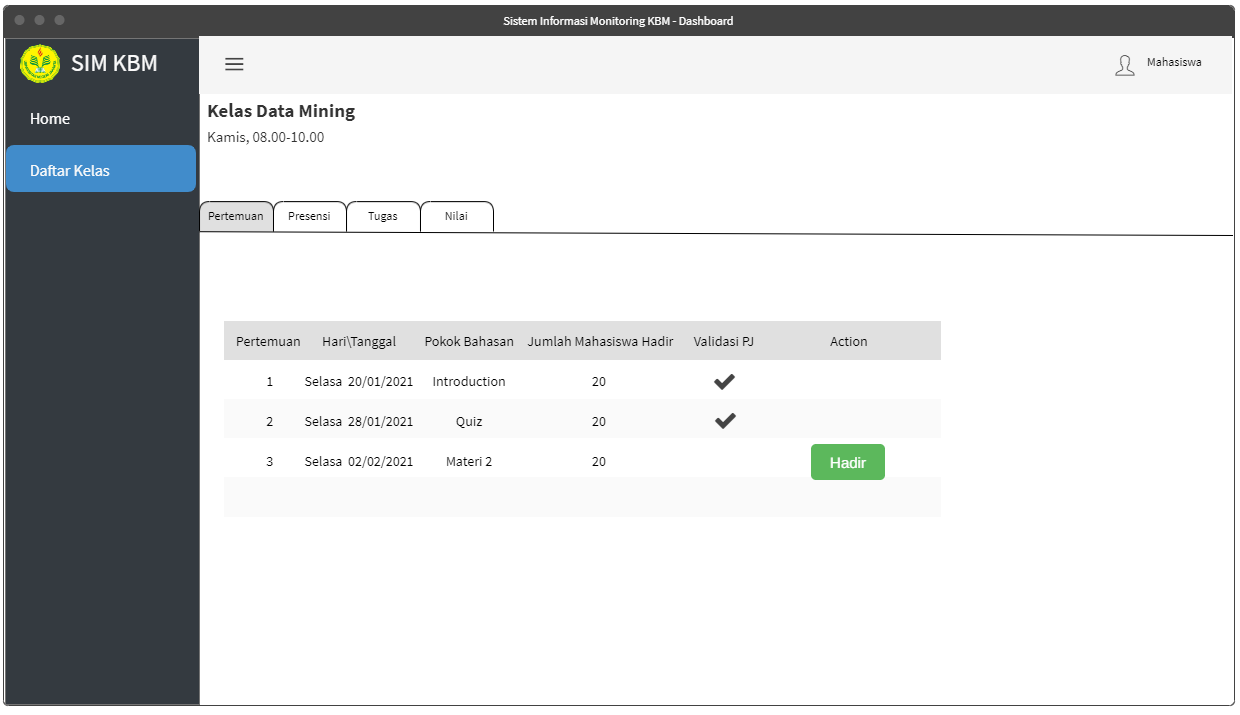
\includegraphics[width=0.8\textwidth]{gambar/mockup/form05_mahasiswa}
	\caption{Desain Halaman Form 05 Pada Mahasiswa }
	\label{fig:form05mhs}
\end{figure}


\subsection{\textit{Class Diagram}}
	Desain \textit{Class Diagram} pada sistem yang dibuat digambarkan dengan mengikuti konsep MVC dimana \textit{class} pada desain dibagi menjadi tiga jenis yaitu \textit{model}, \textit{view}, \textit{controller}. Pada penggunaannya \textit{class} \textit{model} dan \textit{controller} dibuat pada bagian \textit{backend} dengan menggunakan Laravel sedangkan \textit{class view} dibuat pada bagian \textit{frontend} dengan menggunakan \textit{Vue}. Pada diagram berikut ketiga jenis \textit{class} dibedakan dengan menggunakan warna yang berbeda yaitu biru untuk \textit{model}, hijau untuk \textit{view}, dan merah untuk \textit{controller}. Desain \textit{class diagram} pada sistem dapat dilihat pada gambar \ref{fig:classdiagram}

\begin{figure}[H]
	\centering
	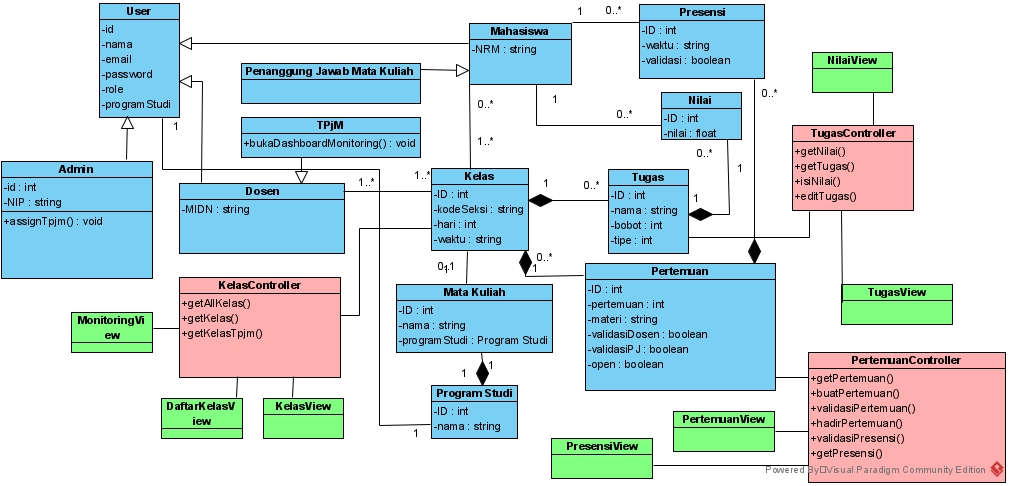
\includegraphics[width=1\textwidth]{gambar/diagram/Class Diagram Fix}
	\caption{Desain Class Diagram}
	\label{fig:classdiagram}
\end{figure}


\subsection{\textit{Entity Relationship Diagram}}
	Desain \textit{Entity Relationship Diagram} pada sistem ini dibuat menggambarkan setiap entitas yang digunakan dalam sistem dan relasinya pada \textit{database} dan pada \textit{web service} SIAKAD yang digunakan. Pada ERD tersebut terdapat sebelas entitas dimana enam diantaranya didapatkan dari \textit{web service} dan lima lainnya berada pada \textit{database} sistem ini sendiri. Entitas yang dibuat dan disimpan pada \textit{database} adalah entitas MahasiswaKelas. Absen, Pertemuan, Nilai, dan Tugas. Entitas MahasiswaKelas merupakan \textit{pivot} antara relasi mahasiswa dan kelas yang disimpan karena menyimpan informasi tambahan selain yang didapatkan dari \textit{webservice} yaitu nilai dan \textit{role} penanggung jawab. Entitas Pertemuan dan Absen yang menghubungkan antara mahasiswa dan kelas merupakan entitas yang menggambarkan form 05 dan 06. Desain ERD pada sistem dapat dilihat pada gambar \ref{fig:erd}

\begin{figure}[h!]
	\centering
	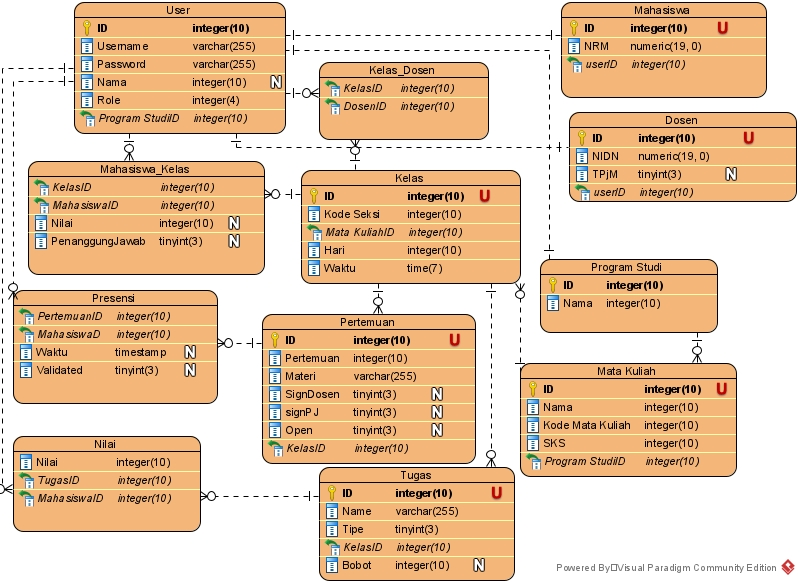
\includegraphics[width=1\textwidth]{gambar/diagram/Entity Relationship Diagram2}
	\caption{Desain Entity Relationship Diagram}
	\label{fig:erd}
\end{figure}

\section{Analisis Risiko}
	Pada fase selanjutnya, penulis melakukan analisis risiko yang dapat terjadi pada pengembangan perangkat lunak, dan mencoba mencari solusi yang dapat dilakukan untuk menangani risiko tersebut. Risiko-risiko yang telah teridentifikasi adalah sebagai berikut:
\begin{enumerate}
	\item Penulis tidak memiliki akses \textit{web service} SIAKAD sebagai dosen. 
	\item Relasi basis data yang tidak lengkap karena menggunakan data dari SIAKAD dan tidak menyimpan kembali ke basis data sistem.
	\item Tidak diberikannya dokumentasi dari \textit{web service} SIAKAD
\end{enumerate}
Setelah risiko yang mungkin terjadi teridentifikasi, penulis mendapat beberapa solusi yaitu:
\begin{enumerate}
	\item Meminta dibuatkan akun dosen dan kelas \textit{dummy} untuk melakukan pengembangan pada sisi dosen.
	\item Menggunakan \textit{query} manual untuk mengakses relasi pada basis data.
	\item Membuat list kebutuhan \textit{web service} dan berkomunikasi dengan pihak UPT TIK terkait \textit{web service} yang dibutuhkan.
\end{enumerate}

\section{Pengembangan}
	Pada fase pengembangan, penulis melakukan proses pengkodean sekaligus pengujian fitur yang dikembangkan. Hasil dari fase ini adalah perangkat lunak sesuai dengan tujuan yang telah ditentukan. Sebagai fase pertama penulis mulai dengan membuat basis data yang dibutuhkan, lalu membuat \textit{backend} beserta hubungannya dengan \textit{web service} SIAKAD, dan membuat \textit{frontend} atau tampilan.

\section{Evaluasi}
	Pada fase evaluasi, penulis melakukan \textit{review} atas iterasi yang telah dilakukan dan merencanakan iterasi yang selanjutnya. Untuk iterasi selanjutnya penulis akan mempersingkat waktu iterasi dengan menyelesaikan iterasi tanpa menunggu berakhirnya minggu kedua ketika semua tujuan iterasi sudah tercapai. Pada iterasi selanjutnya penulis akan mengembangkan sisi dosen dan menyempurnakan sisi mahasiswa yang telah dibuat.














\begin{comment}
\section{Desain Sistem}
Dalam tahapan ini, penulis membuat desain atau \textit{blueprint} dengan menggunakan UML(\textit{Unified Modelling Language}) dari hasil analisis kebutuhan pada tahap sebelumnya. Diagram-diagram yang dibuat oleh penulis adalah \textit{Use Case Diagram}, \textit{Activity Diagram}, dan \textit{Class Diagram}. Selain dari diagram-diagram UML tersebut, penulis juga membuat desain \textit{Entity Relationship Diagram} dan \textit{mockup} dari tampilan antar muka program. Penulis membuat semua diagram-diagram berikut dengan menggunakan Visual Paradigm.

\subsection{\textit{Use Case Diagram}}
	\textit{Use Case Diagram} menggambarkan interaksi apa saja yang dapat dilakukan oleh setiap jenis \textit{user} yang ada pada sistem yang dikembangkan oleh penulis. Pada sistem yang dibuat terdapat 5 aktor yaitu Mahasiswa, Penanggung Jawab Mata Kuliah , Dosen, TPjM, dan admin. Kelima aktor tersebut dapat digeneralisasi menjadi aktor \textit{User} dimana aktor \textit{User} harus melakukan \textit{login} sebelum mengakses sistem. Desain Use Case Diagram untuk sistem yang akan dibuat ada pada pada Gambar \ref{fig:form05}.
	
	Aktor Mahasiswa dapat melihat detail kelas-kelas yang diambil seperti presensi dan nilai setiap mahasiswa pada kelas tersebut dan mengisi presensi pertemuan yang sedang berlangsung.

	Aktor Penanggung Jawab Mata Kuliah dapat digeneralisasi menjadi aktor Mahasiswa sehingga mendapat wewenang yang sama seperti aktor Mahasiswa. Aktor penanggung jawab mata kuliah juga dapat mengisi form 05 atau memvalidasi form 05 yang telah dibuat oleh dosen dan memvalidasi presensi form 06 mahasiswa lain.

	Aktor Dosen memiliki wewenang yang hampir sama dengan wewenang khusus penanggung jawab mata kuliah seperti mengisi form 05, memvalidasi form 05, dan memvalidasi presensi harian kelas. Aktor dosen juga memiliki wewenang tambahan seperti membuat tugas, mengisi nilai, dan memilih penanggung jawab pengganti jika penanggung jawab tidak dapat melakukan tugasnya.

	Aktor TPjM dapat digeneralisasi menjadi aktor dosen sehingga memiliki wewenang  aktor dosen dengan tambahan  dapat melihat rangkuman performa semua kelas dan melihat detail kelas-kelas lain di program studi yang tidak diampu olehnya.

	

\begin{figure}[H]
	\centering
	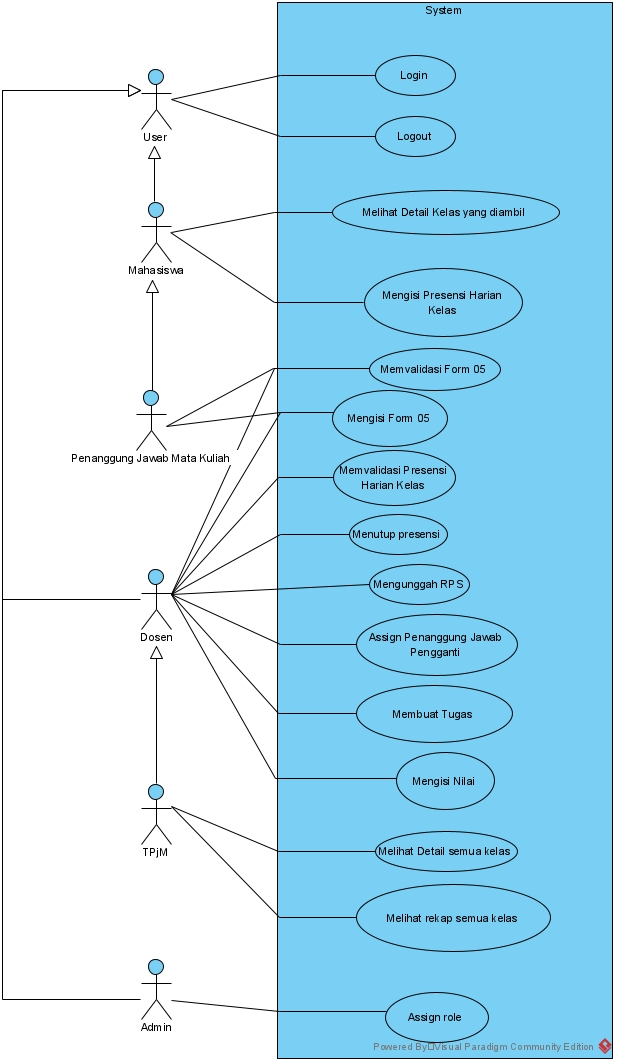
\includegraphics[width=0.8\textwidth]{gambar/diagram/Use Case Diagram}
	\caption{Desain \textit{Use Case Diagram}}
	\label{fig:form05}
\end{figure}

Aktor admin adalah aktor yang dapat mengganti \textit{role user-user} lainnya jika terjadi perubahan. Aktor admin juga bertanggung jawab untuk melakukan \textit{import} data pada awal semester.

\subsection{\textit{Activity Diagram}}
	\textit{Acitivity Diagram} menggambarkan bagaimana alur menjalankan aktivitas yang ada pada sistem. Pada desain sistem ini, dibuat beberapa diagram yang menggambarkan aktivitas-aktivitas utama yang dapat dilakukan pada sistem ini, yaitu mengisi presensi, memvalidasi form, membuat tugas, mengunggah nilai, mengunggah rps, dan memvalidasi presensi.

	Pada gambar \ref{fig:activity1} menggambarkan aktivitas mengunggah RPS dan menambah form 05 yang dapat dilakukan oleh dosen. Dosen diharuskan untuk mengunggah RPS pada pertemuan awal perkuliahan untuk dapat diakses oleh mahasiswa yang mengambil mata kuliah tersebut dan Tim Penjamin Mutu sebagai bahan evaluasi kesesuaian jalannya mata kuliah dengan RPS. Jika pada mata kuliah tersebut sudah memiliki RPS, dosen bisa langsung menambahkan form 05 dan memulai kelas. Form 05 dibutuhkan untuk membuka kesempatan mahasiswa mengisi presensi pertemuan tersebut.

\begin{figure}[h!]
	\centering
	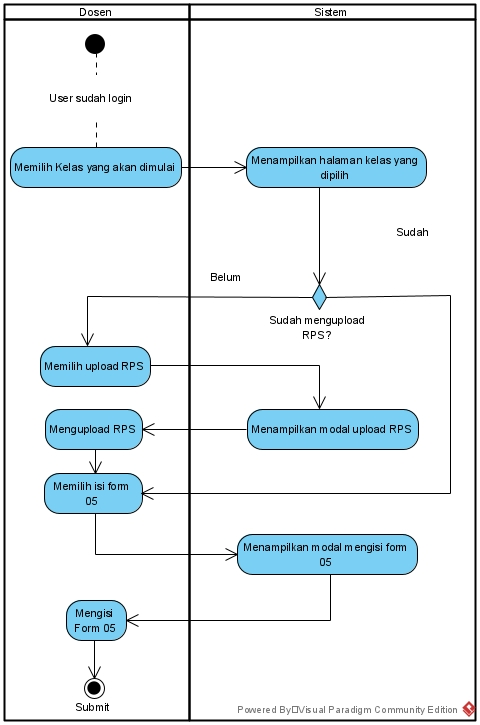
\includegraphics[width=0.7\textwidth]{gambar/diagram/Mengunggah RPS dan Menambah Form 05}
	\caption{\textit{Activity} Mengunggah RPS dan Menambah Form 05}
	\label{fig:activity1}
\end{figure}

	Pada gambar \ref{fig:activity2} menggambarkan aktivitas membuat tugas dan mengunggah nilai yang dapat dilakukan oleh dosen. Dosen dapat membuat tugas dengan cara menekan tombol tambah tugas dan mengisi nama tugas, tanggal, dan tipe tugas. Tipe tugas merupakan pilihan antara tugas, UTS, dan UAS. Tanggal tugas merupakan tanggal tugas tersebut diberikan dan dapat diubah jika tugas tersebut sudah diberikan kepada mahasiswa sebelumnya dan baru dimasukkan ke sistem. Dosen dapat mengunggah nilai dengan cara mengunduh \textit{template} nilai yang merupakan \textit{file} yang sudah berisi tabel nama-nama mahasiswa dan kolom-kolom kosong untuk nilai-nilai tugas, UTS, dan UAS. Dosen dapat mengisi file excel tersebut lalu diunggah kembali ke sistem untuk memperbarui nilai pada sistem.

\begin{figure}[h!]
	\centering
	\includegraphics[width=0.7\textwidth]{gambar/diagram/Membuat Tugas dan Mengunggah Nilai}
	\caption{\textit{Activity} Membuat Tugas dan Mengunggah Nilai}
	\label{fig:activity2}
\end{figure}

	Pada gambar \ref{fig:activity3} menggambarkan aktivitas mengisi presensi yang dapat dilakukan oleh mahasiswa dan memvalidasi form 05 yang dapat dilakukan oleh penanggung jawab mata kuliah. Mahasiswa dapat mengisi presensi dengan cara membuka halaman kelas yang sedang berlangsung dan menekan tombol Hadir. Presensi mahasiswa tersebut akan menunggu validasi oleh dosen untuk dianggap valid dan terekam oleh sistem. Penanggung Jawab Mata Kuliah diharuskan melakukan validasi form 05 yang telah dibuat oleh dosen dengan cara menekan tombol validasi pada tabel form 05 tersebut.

\begin{figure}[h!]
	\centering
	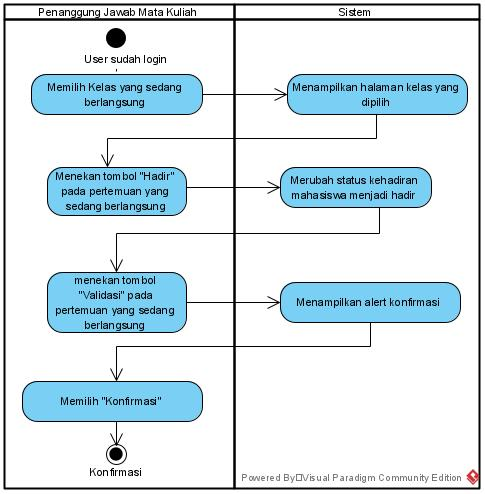
\includegraphics[width=0.7\textwidth]{gambar/diagram/Mengisi Presensi dan Memvalidasi Form 05}
	\caption{\textit{Activity} Mengisi Presensi dan Memvalidasi Form 05}
	\label{fig:activity3}
\end{figure}

	Pada gambar \ref{fig:activity4} menggambarkan aktivitas memilih penanggung jawab pengganti yang dapat dilakukan oleh dosen jika penanggung jawab mata kuliah tidak hadir pada pertemuan yang sedang berlangsung untuk memvalidasi form 05 yang telah dibuat. Penanggung jawab pengganti bersifat sementara dan hanya berlaku pada pertemuan tersebut.

\begin{figure}[h!]
	\centering
	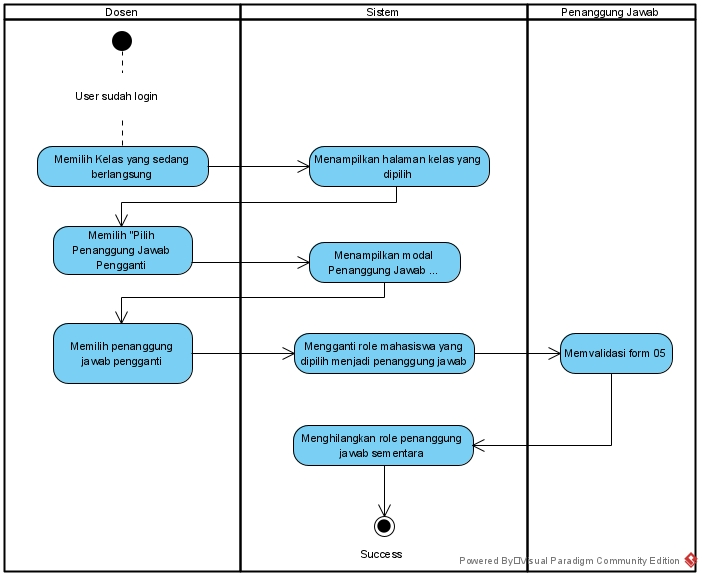
\includegraphics[width=0.7\textwidth]{gambar/diagram/Assign Penanggung Jawab Pengganti}
	\caption{\textit{Activity} Memilih Penanggung Jawab Pengganti}
	\label{fig:activity4}
\end{figure}
	
	Pada gambar \ref{fig:activity6} menggambarkan aktivitas mengganti \textit{role user} yang dapat dilakukan oleh admin. Aktivitas ini utamanya digunakan untuk mengganti \textit{role} TPjM yang dapat berganti setiap tahunnya.

	Pada gambar \ref{fig:activity5} menggambarkan aktivitas memvalidasi presensi yang dapat dilakukan oleh dosen. Dosen harus memvalidasi presensi mahasiswa agar presensi tersebut valid dan terekam oleh sistem. Dosen dapat memilih untuk memvalidasi semua presensi yang sudah diisi oleh mahasiswa atau memilih presensi yang tidak valid dengan cara membatalkan tanda centang \textit{checkbox} pada \textit{list} presensi yang akan divalidasi.

\begin{figure}[H]
	\centering
	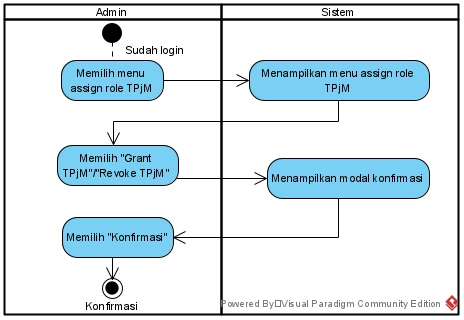
\includegraphics[width=0.7\textwidth]{gambar/diagram/Admin Assign Role}
	\caption{\textit{Activity} Mengganti \textit{role user}}
	\label{fig:activity6}
\end{figure}

\begin{figure}[H]
	\centering
	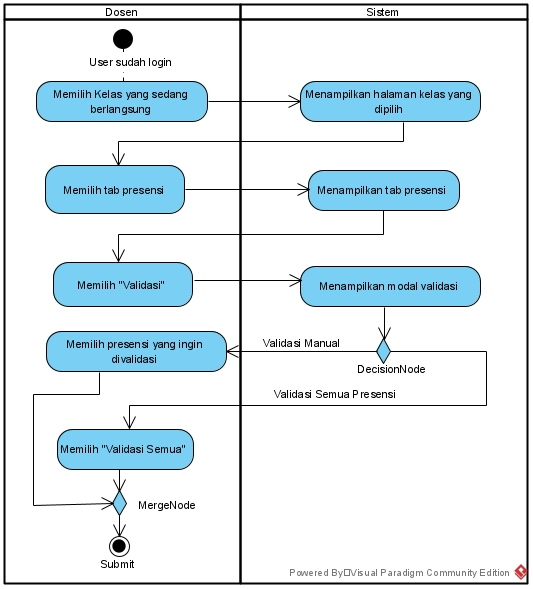
\includegraphics[width=0.7\textwidth]{gambar/diagram/Memvalidasi presensi}
	\caption{\textit{Activity} Memvalidasi Presensi}
	\label{fig:activity5}
\end{figure}



\subsection{\textit{Class Diagram}}
	Desain \textit{Class Diagram} pada sistem yang dibuat digambarkan dengan mengikuti konsep MVC dimana \textit{class} pada desain dibagi menjadi tiga jenis yaitu \textit{model}, \textit{view}, \textit{controller}. Pada penggunaannya \textit{class} \textit{model} dan \textit{controller} dibuat pada bagian \textit{backend} dengan menggunakan Laravel sedangkan \textit{class view} dibuat pada bagian \textit{frontend} dengan menggunakan \textit{Vue}. Pada diagram berikut ketiga jenis \textit{class} dibedakan dengan menggunakan warna yang berbeda yaitu biru untuk \textit{model}, hijau untuk \textit{view}, dan merah untuk \textit{controller}. Desain \textit{class diagram} pada sistem dapat dilihat pada gambar \ref{fig:classdiagram}

\begin{figure}[H]
	\centering
	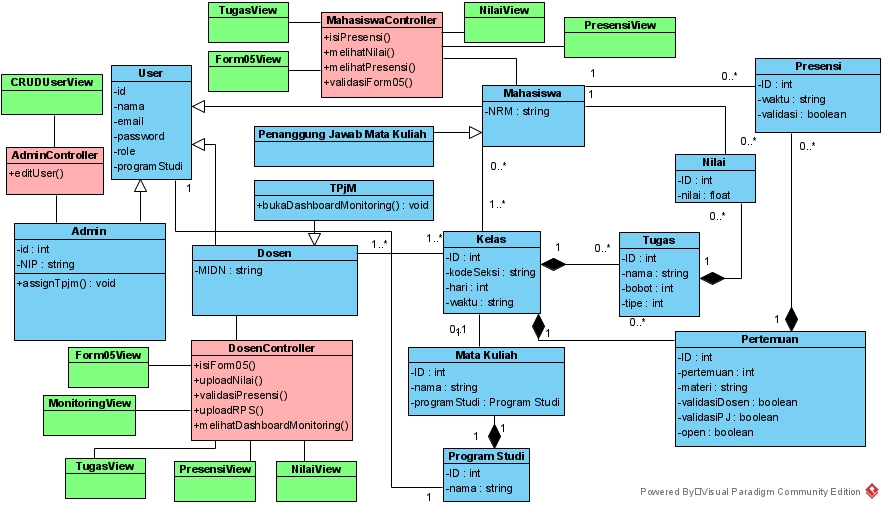
\includegraphics[width=1\textwidth]{gambar/diagram/Class Diagram}
	\caption{Desain Class Diagram}
	\label{fig:classdiagram}
\end{figure}

\subsection{\textit{Entity Relationship Diagram}}
	Desain \textit{Entity Relationship Diagram} pada sistem ini dibuat menggambarkan setiap entitas yang digunakan dalam sistem dan relasinya pada \textit{database} dan pada \textit{web service} SIAKAD yang digunakan. Pada ERD tersebut terdapat sebelas entitas dimana enam diantaranya didapatkan dari \textit{web service} dan lima lainnya berada pada \textit{database} sistem ini sendiri. Entitas yang dibuat dan disimpan pada \textit{database} adalah entitas MahasiswaKelas. Absen, Pertemuan, Nilai, dan Tugas. Entitas MahasiswaKelas merupakan \textit{pivot} antara relasi mahasiswa dan kelas yang disimpan karena menyimpan informasi tambahan selain yang didapatkan dari \textit{webservice} yaitu nilai dan \textit{role} penanggung jawab. Entitas Pertemuan dan Absen yang menghubungkan antara mahasiswa dan kelas merupakan entitas yang menggambarkan form 05 dan 06. Desain ERD pada sistem dapat dilihat pada gambar \ref{fig:erd}

\begin{figure}[h!]
	\centering
	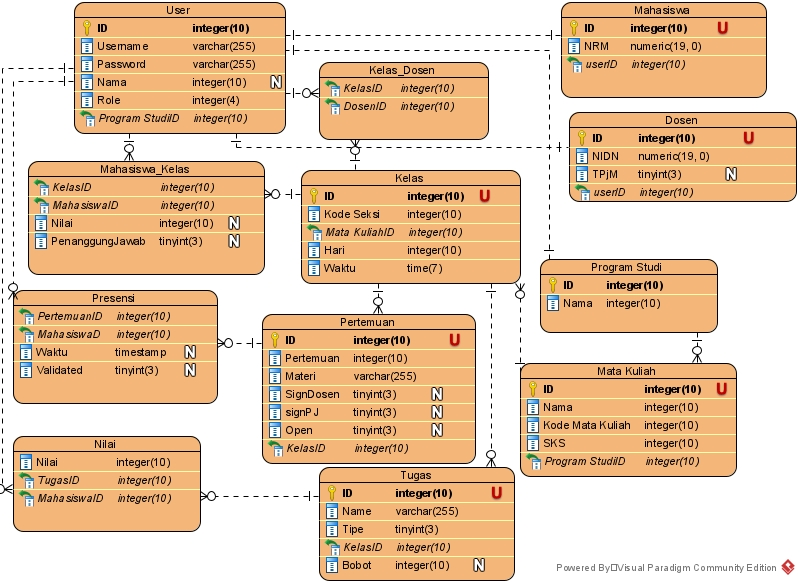
\includegraphics[width=1\textwidth]{gambar/diagram/Entity Relationship Diagram2}
	\caption{Desain Entity Relationship Diagram}
	\label{fig:erd}
\end{figure}

\subsection{Rancangan Tampilan Antarmuka Program}
	Pada rancangan tampilan antar muka program, penulis membuat desain awal dengan menggunakan \textit{tools online}. Pada halaman \textit{login} yang dapat dilihat pada gambar \ref{fig:login}, user mengisi email dan \textit{password} yang terdaftar pada \textit{web service} SIAKAD.

\begin{figure}[h!]
	\centering
	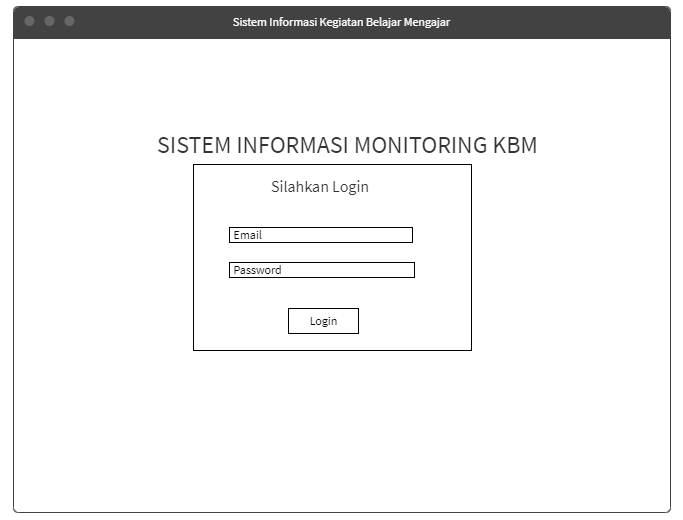
\includegraphics[width=0.8\textwidth]{gambar/mockup/login}
	\caption{Desain Halaman \textit{Login}}
	\label{fig:login}
\end{figure}

Setelah \textit{user} berhasil melakukan \textit{login}, \textit{user} akan dibawa ke halaman \textit{dashboard} dengan menu yang sedikit berbeda bagi setiap jenis \textit{user}. Pada \textit{user} mahasiswa yang dapat dilihat pada gambar \ref{fig:dashboard}, menu yang akan ditampilkan adalah \textit{Home}, Rekap Presensi, dan daftar kelas yang diambil oleh mahasiswa tersebut. Pada \textit{user} dosen, menu yang akan ditampilkan adalah \textit{Home} dan daftar kelas yang diampu oleh dosen tersebut. Pada \textit{user} TPjM menu tambahan akan ditampilkan berupa \textit{Monitoring}.

\begin{figure}[h!]
	\centering
	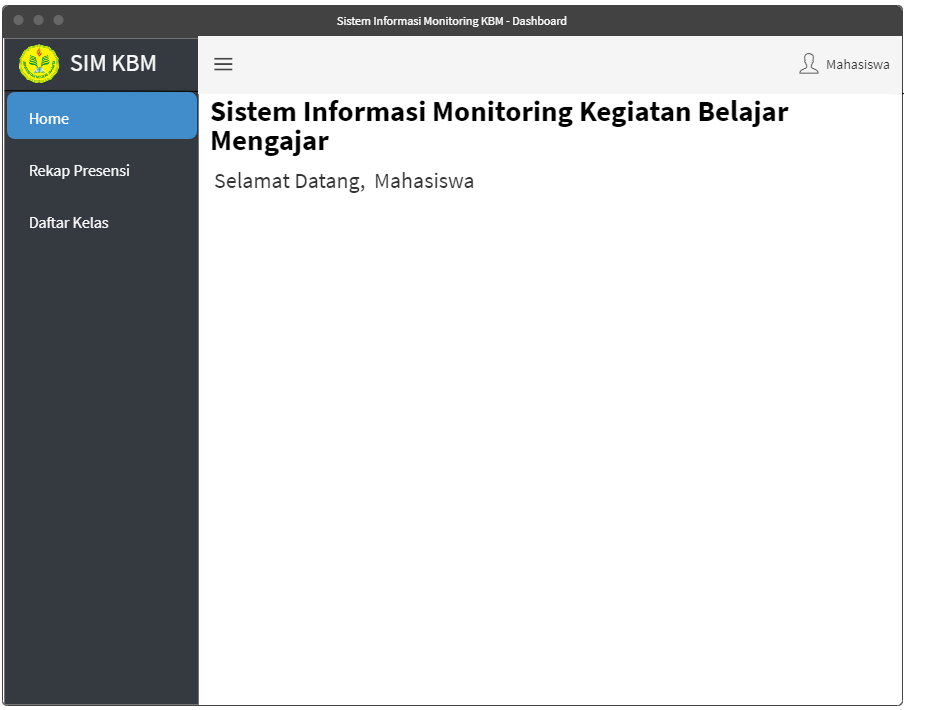
\includegraphics[width=0.8\textwidth]{gambar/mockup/home_mahasiswa}
	\caption{Desain Halaman \textit{Dashboard} Pada mahasiswa}
	\label{fig:dashboard}
\end{figure}

Pada menu Rekap Presensi yang dapat dilihat pada gambar \ref{fig:rekap}, mahasiswa dapat melihat rekap dari presensi setiap mata kuliah yang diambil yang tergabung menjadi satu. Pada menu \textit{monitoring} yang dapat dilihat pada gambar \ref{fig:monitoring}, TPjM dapat melihat daftar semua kelas yang ada pada program studi dan jumlah pertemuan yang telah berjalan. TPjM juga dapat membuka halaman kelas tersebut untuk melihat informasi di dalamnya hanya untuk melakukan monitoring tanpa bisa berinteraksi kecuali jika kelas tersebut juga diampu oleh TPjM tersebut.

\begin{figure}[h!]
	\centering
	\includegraphics[width=0.8\textwidth]{gambar/mockup/rekap_presensi}
	\caption{Desain Halaman Rekap Presensi}
	\label{fig:rekap}
\end{figure}

\begin{figure}[h!]
	\centering
	\includegraphics[width=0.8\textwidth]{gambar/mockup/monitoring}
	\caption{Desain Halaman \textit{Monitoring}}
	\label{fig:monitoring}
\end{figure}

Menu Daftar Kelas merupakan menu yang digunakan untuk membuka halaman kelas yang diambil. Halaman Daftar Kelas dapat dilihat pada gambar \ref{fig:daftarkelas}. Menu kelas terdapat empat bagian \textit{tab} di dalamnya, yaitu Pertemuan, Presensi, Tugas, dan Nilai. Pada \textit{tab} pertemuan yang dapat dilihat pada gambar \ref{fig:form05dosen} dosen dapat menambah pertemuan, memvalidasi form yang dibuat oleh penanggung jawab, memvalidasi presensi mahasiswa, dan mengisi pokok bahasan yang dibahas pada pertemuan tersebut. Setelah pertemuan sudah dibuat dan mahasiswa sudah mengisi presensi dosen juga bisa memvalidasi presensi mahasiswa tersebut. Pada \textit{tab} ini mahasiswa dapat memilih Hadir untuk mengisi presensi pada pertemuan tersebut yang bisa dilihat pada gambar \ref{fig:form05mhs}. Penanggung jawab mata kuliah memiliki fungsi yang sama dengan mahasiswa dan dosen.

\begin{figure}[h!]
	\centering
	\includegraphics[width=0.8\textwidth]{gambar/mockup/daftar_kelas}
	\caption{Desain Halaman Daftar Kelas}
	\label{fig:daftarkelas}
\end{figure}

\begin{figure}[h!]
	\centering
	\includegraphics[width=0.8\textwidth]{gambar/mockup/form05_dosen}
	\caption{Desain Halaman Form 05 Pada Dosen}
	\label{fig:form05dosen}
\end{figure}

\begin{figure}[h!]
	\centering
	\includegraphics[width=0.8\textwidth]{gambar/mockup/form05_mahasiswa}
	\caption{Desain Halaman Form 05 Pada Mahasiswa }
	\label{fig:form05mhs}
\end{figure}



Pada \textit{tab} presensi yang dapat dilihat pada gambar \ref{fig:presensi}, sistem menampilkan tabel presensi dengan format form 06 dimana setiap presensi yang terekam valid akan ditandai dengan tanda centang, dan presensi kosong akan ditandai dengan tanda silang.

\begin{figure}[h!]
	\centering
	\includegraphics[width=0.8\textwidth]{gambar/mockup/form06_presensi}
	\caption{Desain Halaman Presensi}
	\label{fig:presensi}
\end{figure}

Pada \textit{tab} tugas yang dapat dilihat pada gambar \ref{fig:tugas}, dosen dapat menambah tugas yang diberikan pada mahasiswa atau mengubah tugas yang sudah dibuat sebelumnya. Pada \textit{tab} ini mahasiswa tidak dapat berinteraksi dan hanya dapat melihat tabel tugas tersebut dengan tambahan informasi yaitu nilai pada tugas yang didapatkan tersebut. Tampilan halaman tugas untuk mahasiswa dapat dilihat pada gambar \ref{fig:tugasmhs}

\begin{figure}[h!]
	\centering
	\includegraphics[width=0.8\textwidth]{gambar/mockup/tugas}
	\caption{Desain Halaman Tugas Pada Dosen}
	\label{fig:tugas}
\end{figure}

\begin{figure}[h!]
	\centering
	\includegraphics[width=0.8\textwidth]{gambar/mockup/tugas_mahasiswa}
	\caption{Desain Halaman Tugas Pada Mahasiswa}
	\label{fig:tugasmhs}
\end{figure}

Pada \textit{tab} nilai yang dapat dilihat pada gambar \ref{fig:nilai}, dosen dapat melihat tabel nilai setiap mahasiswa dan setiap nilai dari nilai tugas, UTS, dan UAS. Pada \textit{tab} ini, dosen dapat mengunduh dan mengunggah nilai untuk memperbarui nilai pada sistem.

\begin{figure}[h!]
	\centering
	\includegraphics[width=0.8\textwidth]{gambar/mockup/nilai}
	\caption{Desain Halaman Nilai Pada Dosen}
	\label{fig:nilai}
\end{figure}

\end{comment}
%END OF SPS

%%!TEX root = ./template-skripsi.tex
%-------------------------------------------------------------------------------
%                            	BAB IV
%               		KESIMPULAN DAN SARAN
%-------------------------------------------------------------------------------

\chapter{HASIL DAN UJI COBA}


\section{Spiral Kedua}		%SPIRAL 2
\subsection{Perencanaan}

\begin{figure}[H]
	\centering
	\includegraphics[width=0.8\textwidth]{gambar/diagram/Use Case Iteration 2}
	\caption{Desain \textit{Use Case Diagram Iterasi Kedua}}
	\label{fig:usecase2nd}
\end{figure}

	Dalam tahap perencanaan spiral 2, penulis kembali membuat desain\textit{ Use Case Diagram}, \textit{Activity Diagram}, dan rancangan tampilan antar muka yang akan menjadi tujuan pengembangan pada iterasi kedua. Pada spiral 2, penulis membuat halaman presensi, tugas, dan nilai untuk dosen. Fungsionalitas yang dibuat adalah memilih penanggung jawab, membuat tugas, menggunggah nilai, dan memvalidasi presensi kehadiran.  

\textbf{A. \textit{Use Case Diagram}}

	Pada Spiral 2, penambahan fitur dapat digambarkan dengan \textit{Use Case Diagram} pada gambar \ref{fig:usecase2nd}. Pada iterasi ini, pengembangan fitur berfokus kepada fungsionalitas pada \textit{user} Dosen seperti memilih penanggung jawab, membuat tugas, memvalidasi presensi kehadiran, dan mengunggah nilai.

\textbf{B. \textit{Activity Diagram}}

\begin{figure}[H]
	\centering
	\includegraphics[width=0.8\textwidth]{gambar/diagram/Memvalidasi presensi}
	\caption{Desain \textit{Activity Diagram Memvalidasi Presensi}}
	\label{fig:actvalidasipresensi}
\end{figure}
	Dari beberapa \textit{Use Case} yang telah dibuat, penulis juga membuat \textit{Activty Diagram} untuk memperjelas alur cara kerja fitur yang dibuat. \textit{Activity Diagram} yang dibuat pada iterasi ini dapat dilihat pada gambar \ref{fig:actvalidasipresensi} dan gambar \ref{fig:acttugasnilai}

\begin{figure}[H]
	\centering
	\includegraphics[width=0.8\textwidth]{gambar/diagram/Membuat tugas dan Mengunggah Nilai}
	\caption{Desain \textit{Activity Diagram Membuat tugas dan Mengunggah Nilai}}
	\label{fig:acttugasnilai}
\end{figure}


\textbf{C. Rancangan Tampilan Antar Muka}

	Pada Spiral 2, penulis juga membuat desain tampilan antar muka yang akan dibuat yaitu rancangan tampilan halaman Presensi, Tugas, dan Nilai. Pada gambar \ref{fig:mockpresensi} dapat dilihat desain tampilan halaman presensi dimana pengguna dapat melihat daftar mahasiswa yang mengikuti kelas dan presensi pada setiap pertemuannya. Pada gambar \ref{fig:mocktugas} dapat dilihat desain tampilan halaman tugas dimana dosen dapat membuat, menyunting, atau menghapus tugas. Pada tabel tugas, terdapat nama tugas, tanggal,  bobot, dan tipe. Bobot adalah bobot nilai tugas dalam persen sedangkan tipe adalah tipe tugas yang dapat berupa Tugas, UTS, atau UAS. Pada gambar \ref{fig:mocknilai} adalah desain tampilan halaman nilai yang hanya dapat dilihat oleh dosen. Pada tampilan ini dosen dapat mengunduh \textit{excel} nilai untuk mulai mengisi nilai, setelah \textit{file excel} sudah diisi dengan nilai, \textit{file} tersebut dapat diunggah kembali untuk memasukkan nilai ke dalam sistem.

\begin{figure}[h!]
	\centering
	\includegraphics[width=1\textwidth]{gambar/mockup/form06_presensi}
	\caption{Desain Tampilan Halaman Presensi}
	\label{fig:mockpresensi}
\end{figure}

\begin{figure}[h!]
	\centering
	\includegraphics[width=1\textwidth]{gambar/mockup/tugas_dosen}
	\caption{Desain Tampilan Halaman Tugas Pada Dosen}
	\label{fig:mocktugas}
\end{figure}

\begin{figure}[h!]
	\centering
	\includegraphics[width=1\textwidth]{gambar/mockup/nilai_dosen}
	\caption{Desain Tampilan Halaman Nilai Pada Dosen}
	\label{fig:mocknilai}
\end{figure}

\subsection{Analisis Risiko}
	Pada spiral 2, risiko yang didapati penulis ada pada membuat tampilan dan \textit{flow} yang sesuai dan dapat memberikan \textit{User Experience} yang terbaik.
\subsection{Pengembangan}
	Pada fase pengembangan, penulis melakukan proses pengembangan fitur-fitur yang telah direncanakan. Pada pengembangan spiral 2, penulis membuat tampilan halaman-halaman presensi, tugas, dan nilai pada \textit{frontend} dan membuat \textit{model} dan\textit{controller} pada \textit{backend}. Berikut adalah tampilan-tampilan yang telah dibuat pada fase pengembangan ini.

\begin{figure}[h!]
	\centering
	\includegraphics[width=1\textwidth]{gambar/ss/presensi}
	\caption{Tampilan Halaman Presensi}
	\label{fig:sspresensi}
\end{figure}

Pada gambar \ref{fig:sspresensi} adalah halaman \textit{tab} presensi atau form 06. Pada halaman ini terdapat tabel presensi yang berisi daftar mahasiswa dan presensi mahasiswa tersebut pada setiap pertemuan. Kehadiran mahasiswa akan ditandai dengan ikon centang sedangkan ketidakhadiran akan ditandai dengan ikon silang. Pada halaman presensi juga terdapat tombol \textit{reload} pada sisi kanan untuk memperbarui tabel jika ada perubahan.

\begin{figure}[h!]
	\centering
	\includegraphics[width=1\textwidth]{gambar/ss/tugas}
	\caption{Tampilan Halaman Tugas Pada Dosen}
	\label{fig:sstugas}
\end{figure}

\begin{figure}[h!]
	\centering
	\includegraphics[width=1\textwidth]{gambar/ss/tugas_mhs}
	\caption{Tampilan Halaman Tugas Pada Mahasiswa}
	\label{fig:sstugasmhs}
\end{figure}

Pada gambar \ref{fig:sstugas} adalah halaman \textit{tab} tugas pada dosen dan gambar \ref{fig:sstugasmhs} adalah halaman \textit{tab} tugas pada mahasiswa. Pada halaman ini dosen dapat membuat tugas baru, menyunting, dan menghapus tugas yang sudah ada. Pada kolom bobot terdapat jumlah bobot tugas-tugas yang telah dibuat, jika bobot sudah mencapai 100 atau lebih, tulisan tersebut akan menjadi berwarna merah untuk menandakan bobot tugas sudah lengkap. Pada mahasiswa, halaman tugas akan berisi nilai pada masing-masing tugas, dan nilai akhir beserta nilai hurufnya. Pada halaman tugas juga terdapat tombol \textit{reload} pada sisi kanan untuk memperbarui tabel jika ada perubahan.

\begin{figure}[h!]
	\centering
	\includegraphics[width=1\textwidth]{gambar/ss/nilai}
	\caption{Tampilan Halaman Nilai}
	\label{fig:ssnilai}
\end{figure}

Pada gambar \ref{fig:ssnilai} adalah halaman \textit{tab} nilai yang hanya dapat dilihat oleh dosen. Pada halaman ini dosen dapat mengunggah dan mengunduh \textit{excel} nilai.

\subsection{Evaluasi}
	Pada fase evaluasi, penulis kembali melakukan pengujian kembali fitur yang telah dibuat dan melakukan \textit{review} pada kode yang telah dibuat untuk mencari cara implementasi yang lebih baik. Pada fitur nilai, dibutuhkan untuk menerapkan aturan \textit{input} nilai yaitu mahasiswa hanya bisa mendapatkan nilai UAS jika jumlah kehadiran mencapai 80\%. Pada iterasi selanjutnya penulis akan melanjutkan pengembangan dan memperbaiki fitur penanggung jawab pengganti menjadi khusus pada satu pertemuan saja.

\section{Spiral Ketiga}		%SPIRAL 3
\subsection{Perencanaan}
	Pada spiral 3, penulis merencanakan untuk memperbaiki fitur yang telah dievaluasi pada spiral sebelumnya dan menambahkan fitur-fitur baru yaitu menampilkan halaman monitoring untuk TPjM yang menampilkan data-data kelas yang ada dalam satu program studi, fitur unggah dan unduh RPS, rekap presensi mahasiswa, dan halaman admin untuk mengatur \textit{role} TPjM.

\textbf{A. \textit{Use Case Diagram}}

\begin{figure}[h!]
	\centering
	\includegraphics[width=0.8\textwidth]{gambar/diagram/Use Case Iteration 3}
	\caption{Desain \textit{Use Case Diagram Iterasi Ketiga}}
	\label{fig:usecase3rd}
\end{figure}

	Pada Spiral 3, penambahan fitur dapat digambarkan dengan \textit{Use Case Diagram} pada gambar \ref{fig:usecase3rd}. Pada iterasi ini, dilakukan pengembangan fitur pada beberapa aktor, pada mahasiswa ada penambahan rekap presensi dan mengunduh RPS, pada dosen terdapat penambahan mengunggah dan mengunduh RPS. Selain itu ditambahkan tampilan monitoring TPjM yang berupa daftar kelas dalam satu program studi yang merupakan \textit{homebase} dosen yang bersangkutan. Pada iterasi ini ditambahkan juga aktor baru yaitu admin yang memiliki fungsi untuk mengubah \textit{role} TPjM.


\textbf{B. \textit{Activity Diagram}}

	Pada spiral 3, penulis membuat \textit{Activity Diagram} untuk membantu menjelaskan interaksi yang terjadi pada \textit{Use Case}. \textit{Activity Diagram} yang dibuat pada iterasi ini dapat dilihat pada gambar \ref{fig:actadmin}.

\begin{figure}[h!]
	\centering
	\includegraphics[width=0.8\textwidth]{gambar/diagram/Admin Assign Role}
	\caption{Desain \textit{Activity Diagram Admin Assign Role}}
	\label{fig:actadmin}
\end{figure}

\textbf{C. Rancangan Tampilan Antar Muka}

	Pada Spiral 2, penulis membuat desain tampilan antar muka yang akan dibuat yaitu rancangan tampilan halaman admin, rekap presensi, dan halaman monitoring. Pada gambar \ref{fig:mockadmin} dapat dilihat desain tampilan halaman dimana admin dapat mengganti \textit{role} dosen menjadi TPjM atau sebaliknya. Pada gambar \ref{fig:mockrekappresensi} dapat dilihat desain tampilan halaman rekap presensi mahasiswa. Pada gambar \ref{fig:mockmonitoring} dapat dilihat tampilan halaman monitoring dimana TPjM dapat melihat daftar kelas pada program studi \textit{homebase}nya.

\begin{figure}[h!]
	\centering
	\includegraphics[width=1\textwidth]{gambar/mockup/admin_dosen}
	\caption{Desain Tampilan Halaman Admin \textit{Assign Role}}
	\label{fig:mockadmin}
\end{figure}

\begin{figure}[h!]
	\centering
	\includegraphics[width=1\textwidth]{gambar/mockup/rekap_presensi}
	\caption{Desain Tampilan Halaman Rekap Presensi}
	\label{fig:mockrekappresensi}
\end{figure}

\begin{figure}[h!]
	\centering
	\includegraphics[width=1\textwidth]{gambar/mockup/monitoring}
	\caption{Desain Tampilan Halaman Monitoring}
	\label{fig:mockmonitoring}
\end{figure}

\subsection{Analisis Risiko}
	Pada fase ini, penulis mendapatkan hasil analisis yaitu dibutuhkan API SIAKAD tambahan untuk mengambil data semua kelas pada satu program studi dan membuat tampilan kelas tanpa adanya action apa-apa untuk tampilan monitoring TPjM.
\subsection{Pengembangan}
	Pada pengembangan spiral 3, penulis membuat tampilan daftar kelas monitoring TPjM dan rekap presensi dan pada \textit{backend} penulis membuat \textit{import export excel} untuk mengunduh dan mengunggah nilai. Berikut adalah tampilan-tampilan yang telah dibuat pada fase pengembangan ini.

\begin{figure}[h!]
	\centering
	\includegraphics[width=1\textwidth]{gambar/ss/monitoring}
	\caption{Tampilan Halaman Monitoring}
	\label{fig:ssmonitoring}
\end{figure}

Pada gambar \ref{fig:ssmonitoring} adalah tampilan halaman monitoring dimana TPjM dapat melihat daftar kelas yang ada pada program studi, TPjM dapat mengeklik salah satu kelas untuk melihat halaman kelas tersebut. Halaman kelas yang dibuka dari menu monitoring tidak memiliki tombol interaksi apapun kecuali mengunduh RPS dan nilai.

\begin{figure}[h!]
	\centering
	\includegraphics[width=1\textwidth]{gambar/ss/rekap_presensi}
	\caption{Tampilan Halaman Rekap Presensi}
	\label{fig:ssrekappresensi}
\end{figure}

\begin{figure}[h!]
	\centering
	\includegraphics[width=1\textwidth]{gambar/ss/admin}
	\caption{Tampilan Halaman Admin}
	\label{fig:ssadmin}
\end{figure}

\subsection{Evaluasi}
	Pada evaluasi spiral 3, didapatkan kebutuhan untuk melihat data kelas pada semester sebelumnya baik pada mahasiswa, dosen, maupun monitoring. Penulis memutuskan untuk menambah iterasi tambahan untuk memperbaiki detil-detil fitur dan tampilan yang sudah ada dan beberapa perubahan desain dan kebutuhan.

\section{Spiral Keempat}		%SPIRAL 4
\subsection{Perencanaan}
	Pada fase perencanaan spiral 4, penulis menambahkan perizinan mahasiswa, mengubah bobot tugas sekaligus pada halaman nilai untuk mempermudah dosen, dan kebutuhan untuk melihat data pada semester sebelumnya. Selain itu penulis juga memperbaiki beberapa detil tampilan dan fitur-fitur lainnya.

\textbf{A. \textit{Use Case Diagram}}

	Pada spiral 4, penambahan pada i dapat dilihat pada gambar \ref{fig:usecase4th}. Pada gambar tersebut dapat dilihat penambahan \textit{Use Case} pada aktor dosen dan mahasiswa. 

\begin{figure}[h!]
	\centering
	\includegraphics[width=0.8\textwidth]{gambar/diagram/Use Case Iteration 4}
	\caption{Desain \textit{Use Case Diagram Iterasi Keempat}}
	\label{fig:usecase4th}
\end{figure}

\textbf{B. \textit{Activity Diagram}}

	Pada spiral 4, penulis membuat \textit{Activity Diagram} untuk membantu menjelaskan interaksi yang terjadi pada \textit{Use Case}. \textit{Activity Diagram} yang dibuat pada iterasi ini dapat dilihat pada gambar \ref{fig:actperizinan}.

\begin{figure}[h!]
	\centering
	\includegraphics[width=0.8\textwidth]{gambar/diagram/perizinan}
	\caption{Desain \textit{Activity Diagram} Perizinan}
	\label{fig:actperizinan}
\end{figure}

\subsection{Analisis Risiko}
	Pada spiral 4, dikarenakan adanya kebutuhan baru untuk dapat melihat data semester sebelumnya, penulis harus melakukan perubahan pada kode yang sudah ada yang sebelumnya hanya memberikan data dengan semester aktif.
\subsection{Pengembangan}
	Pada pengembangan spiral 4, penulis menambahkan tombol perizinan pada halaman presensi dan tombol Ubah Bobot Tugas pada halaman nilai, untuk mengubah bobot tugas sekaligus untuk mempermudah dosen jika ingin menyesuaikan bobot tugas dan melihat efek perubahan bobot tugas tersebut pada nilai mahasiswa. Penulis juga menambahkan pemilihan semester pada rekap presensi, daftar kelas, dan monitoring untuk melihat data pada semester sebelumnya. 
\subsection{Evaluasi}
	Pada evaluasi spiral terakhir, penulis melakukan \textit{review} pada fitur-fitur yang sudah ada dan memastikan bahwa semuanya sudah berjalan dengan baik dan sesuai kebutuhan. Setelah semua fitur-fitur yang ada telah dievaluasi dan sudah berjalan sesuai dengan desain dan kebutuhan sistem siap untuk dilakukan pengujian oleh pengguna.
%END SPIRAL 


\section{Uji Coba}
	Uji coba pada sistem dilakukan terhadap enam responden mahasiswa yang pernah atau sedang menjadi penanggung jawab kelas dan empat dosen dimana tiga di antaranya merupakan TPjM. Setiap responden akan menguji coba sistem yang telah dikembangkan berdasarkan peran masing-masing responden. Uji coba yang dilakukan menggunakan data yang didapatkan dari hasil sebaran kuesioner \textit{User Acceptance Test}. \textit{User Acceptance Test} bertujuan untuk mengetahui apakah sistem yang dibuat sudah sesuai dengan kebutuhan \textit{user} atau belum. Berikut langkah-langkah pengujian yang akan dilakukan pada sistem informasi Koperasi Mahasiswa Universitas Negeri Jakarta:
\begin{enumerate}
	\item Mahasiswa
	\begin{itemize}
		\item Melakukan \textit{login} menggunakan akun SIAKAD.
		\item Mengunduh RPS.
		\item Membuat pertemuan.
		\item Memvalidasi pertemuan.
		\item Mengisi kehadiran pertemuan.
		\item Melihat data presensi kehadiran kelas.
		\item Melihat data tugas dan perhitungan nilai.
		\item Melihat rekap presensi.
		\item Melihat data semester sebelumnya.
	\end{itemize}
	\item Dosen
	\begin{itemize}
		\item Melakukan \textit{login} menggunakan akun SIAKAD.
		\item Mengolah (membuat, menyunting, menghapus) pertemuan.
		\item Memvalidasi pertemuan.
		\item Memvalidasi presensi kehadiran.
		\item Mengisi perizinan mahasiswa.
		\item Melihat data presensi kehadiran kelas.
		\item Mengolah (membuat, menyunting, menghapus) tugas.
		\item Mengunduh dan mengunggah \textit{excel} nilai.
		\item Memilih penanggung jawab kelas dan penanggung jawab sementara.
		\item Mengunggah dan mengunduh RPS.
		\item Melihat halaman monitoring untuk TPjM.
		\item Melihat data semester sebelumnya.
	\end{itemize}
\end{enumerate}

Pengujian yang dilakukan terdiri dari dua pengujian, yaitu pengujian fungsionalitas dan pengujian kebergunaan atau \textit{usablity}. Pada pengujian fungsional, sistem penilaian yang digunakan berdasarkan pada pilihan: \\

\begin{tabular}{lll}
S& : Setuju\\
TS& : Tidak Setuju\\
\\
\end{tabular}

Pada pengujian kebergunaan (\textit{usability}), sistem penilaian yang digunakan adalah skala likert. Skala likert adalah skala yang terdiri dari serangkaian pernyataan yang menjelaskan sikap responden terhadap objek penelitian. Setiap pernyataan terdapat lima poin dari skala "sangat tidak setuju" hingga "sangat tidak setuju" \citep{Ahyar2020}. Setelah didapatkan seluruh data penilaian dari responden, nilai tersebut dikalkulasikan sesuai sistem penilaian berikut:

\begin{itemize}
	\item Nilai Total

		Nilai total adalah jumlah keseluruhan yang didadapat dari tiap pernyataan atau dapat ditulis menjadi: \\
		\(Nilai Total = (jumlah \times skorSS) + (jumlah \times skorS) + (jumlah \times skorC) + (jumlah \times skorTS) + (jumlah \times skorSTS)\)
	\item Persentase Kelayakan
		Persentase kelayakan adalah persentase nilai rata-rata yang didapatkan dengan cara membagi nilai total dengan skor maksimal.  Skor maksimal adalah nilai maksimal skala likert yang dikalikan dengan jumlah pernyataan. Perhitungan tersebut dapat ditulis menjadi: \\
		\(Persentase Kelayakan(\%) = \frac{NilaiTotal}{SkorMaksimal}\times100\)
\end{itemize}

Persentase kelayakan yang sudah didapatkan akan dibandingkan dengan skor pada skala likert untuk menarik kesimpulan akhir dari hasil pengujian. Berikut model skor skala likert:\\

\begin{tabular}{lll}
1. Sangat Kurang Sesuai& = 0\% - 20\%\\
2. Kurang Sesuai& = 21\% - 40\%\\
3. Cukup Sesuai& = 41\% - 60\%\\
4. Sesuai& = 61\% - 80\%\\
5. Sangat Sesuai& = 81\% - 100\%\\
\\
\end{tabular}

\section{Hasil Uji Coba}
Berdasarkan hasil uji coba \textit{User Acceptance Test} yang dilakukan terhadap enam responden mahasiswa dan empat responden dosen, diperoleh hasil uji coba sebagai berikut:

\subsection{Pengujian Oleh Mahasiswa}
Pengujian oleh mahasiswa dilakukan oleh enam mahasiswa yang mencakup empat mahasiswa program studi Ilmu Komputer dan dua mahasiswa pendidikan matematika . Berikut merupakan hasil penilaian \textit{User Acceptance Test} yang diberikan Mahasiswa mengenai fungsionalitas dan kebergunaan:

\begin{table}[h!]
\centering
\def\arraystretch{1.5}
\caption{Hasil Uji Fungsionalitas Pada Mahasiswa}
\label{tab:fungsiomhs}
\begin{tabular} { | >{\centering\arraybackslash}m{1em} | >{\raggedright\arraybackslash}m{22em} | >{\centering\arraybackslash}m{3.7em} | >{\centering\arraybackslash}m{3.7em} | }
	\hline
	\multirow{2}{*}{\textbf{No.}} & \multicolumn{1}{c|}{\multirow{2}{*}{\textbf{Pernyataan}}} & \multicolumn{2}{c|}{\textbf{Jawaban Responden}} \\ 
	\cline{3-4} && \textbf{TS} & \textbf{S}\\
	\hline

	1 & Fitur \textit{login} berjalan dengan baik. & 0 & 6 \\ \hline
	2 & Fitur daftar kelas dan filter semester berjalan dengan baik. & 0 & 6 \\ \hline
	3 & Fitur mengunduh rps berjalan dengan baik. & 0 & 6 \\ \hline
	4 & Fitur mengelola (membuat dan memvalidasi) pertemuan berjalan dengan baik. & 0 & 6 \\ \hline
	5 & Fitur hadir dan validasi presensi berjalan dengan baik. & 0 & 6 \\ \hline
	6 & Fitur tabel presensi berjalan dengan baik. & 0 & 6 \\ \hline
	7 & Fitur tugas dan nilai berjalan dengan baik. & 0 & 6 \\ \hline
	8 & Fitur rekap presensi dan filter semester berjalan dengan baik. & 0 & 6 \\ \hline
	9 & Fitur \textit{logout} berjalan dengan baik. & 0 & 6 \\ \hline
	\multicolumn{2}{|c|}{Total} & 0 & 54 \\ \hline
	\multicolumn{2}{|c|}{Persentase Jawaban} & \textbf{0\%} & \textbf{100\%} \\ \hline

\end{tabular}
\end{table}

Berdasarkan hasil uji coba fungsionalitas dari kuisioner UAT pada pengguna mahasiswa, didapatkan persentase jawaban sebesar 100\%. Dari hasil persentase jawaban yang didapatkan, dapat dikatakan bahwa sistem informasi monitoring kegiatan belajar mengajar ini berjalan dengan baik dan sesuai dengan yang diharapkan.

%\begin{table}[h!]
%\centering
%\def\arraystretch{1.5}

\begin{longtable}[h!] { | >{\centering\arraybackslash}m{1em} | >{\raggedright\arraybackslash}m{22em} | >{\centering\arraybackslash}m{1em} | >{\centering\arraybackslash}m{1em} | >{\centering\arraybackslash}m{1em} | >{\centering\arraybackslash}m{1em} | >{\centering\arraybackslash}m{1em} | }
\caption{Hasil Uji Kebergunaan Pada Mahasiswa}
\label{tab:usabilmhs}\\
	\hline
	\multirow{2}{*}{\textbf{No.}} & \multicolumn{1}{c|}{\multirow{2}{*}{\textbf{Pernyataan}}} & \multicolumn{5}{c|}{\textbf{Jawaban Responden}} \\ 
	\cline{3-7} && \textbf{1} & \textbf{2} & \textbf{3} & \textbf{4} & \textbf{5}\\
	\hline

	1 & Fitur hadir dan validasi presensi mudah dimengerti. & 0 & 0 & 0 & 1 & 5 \\ \hline
	2 & Fitur mengelola (membuat dan memvalidasi) pertemuan mudah dimengerti. & 0 & 0 & 1 & 1 & 4 \\ \hline
	3 & Fitur rekap presensi dan filter semester mudah dimengerti. & 0 & 0 & 0 & 1 & 5 \\ \hline
	4 & Sistem ini mudah digunakan. & 0 & 0 & 0 & 1 & 5 \\ \hline
	5 & Sistem ini nyaman digunakan. & 0 & 0 & 0 & 2 & 4 \\ \hline
	6 & Sistem ini dapat membantu mahasiswa dalam proses kegiatan belajar mengajar. & 0 & 0 & 0 & 1 & 5 \\ \hline
	\multicolumn{2}{|c|}{Total} & 0 & 0 & 1 & 7 & 28 \\ \hline

\end{longtable}
%\end{table}

\(Nilai Total = (0 \times 1) + (0 \times 2) + (1 \times 3) + (7 \times 4) + (28 \times 5) = 171\).
\indent \(Persentase Kelayakan(\%) = \frac{171}{180}\times100=95\%\). \\
\indent Berdasarkan hasil uji coba kebergunaan pada pengguna mahasiswa, didapatkan persentase kelayakan senilai 95\%. Dari hasil persentase kelayakan yang didapatkan, dapat dikatakan bahwa sistem informasi monitoring kegiatan belajar mengajar ini mendapat predikat sesuai dalam aspek kebergunaan sistem.

\subsection{Pengujian Oleh Dosen}
Pengujian oleh dosen dilakukan oleh empat dosen dari masing-masing program studi Ilmu Komputer, Pendidikan Matematika, Matematika, dan Statistika dimana tiga diantaranya merupakan TPjM. Berikut merupakan hasil penilaian \textit{User Acceptance Test} yang diberikan dosen mengenai fungsionalitas dan kebergunaan:

%\begin{table}[h!]
%\centering
%\def\arraystretch{1.5}
\begin{longtable} { | >{\centering\arraybackslash}m{1em} | >{\raggedright\arraybackslash}m{22em} | >{\centering\arraybackslash}m{3.7em} | >{\centering\arraybackslash}m{3.7em} | }
\caption{Hasil Uji Fungsionalitas Pada Dosen}
\label{tab:fungsiodsn} \\
	\hline
	\multirow{2}{*}{\textbf{No.}} & \multicolumn{1}{c|}{\multirow{2}{*}{\textbf{Pernyataan}}} & \multicolumn{2}{c|}{\textbf{Jawaban Responden}} \\ 
	\cline{3-4} && \textbf{TS} & \textbf{S}\\
	\hline

	1 & Fitur login berjalan dengan baik. & 0 & 4 \\ \hline
	2 & Fitur daftar kelas dan filter semester berjalan dengan baik. & 0 & 4 \\ \hline
	3 & Fitur unggah dan unduh RPS berjalan dengan baik. & 0 & 4 \\ \hline
	4 & Fitur pilih penanggung jawab dan penanggung jawab sementara berjalan dengan baik. & 0 & 4 \\ \hline
	5 & Fitur mengelola (membuat, mengubah materi, memvalidasi, dan menghapus) pertemuan berjalan dengan baik. & 0 & 4 \\ \hline
	6 & Fitur tabel presensi berjalan dengan baik. & 0 & 4 \\ \hline
	7 & Fitur validasi  presensi dan perizinan berjalan dengan baik. & 0 & 4 \\ \hline
	8 & Fitur mengelola (membuat, mengyunting, dan menghapus) tugas berjalan dengan baik. & 0 & 4 \\ \hline
	9 & Fitur mengunggah dan mengunduh nilai berjalan dengan baik. & 0 & 4 \\ \hline
	10 & Fitur monitoring dan filter semester berjalan dengan baik (TPjM). & 0 & 3 \\ \hline
	11 & Fitur logout berjalan dengan baik. & 0 & 4 \\ \hline
	\multicolumn{2}{|c|}{Total} & 0 & 43 \\ \hline
	\multicolumn{2}{|c|}{Persentase Jawaban} & \textbf{0\%} & \textbf{100\%} \\ \hline

\end{longtable}
%\end{table}

Berdasarkan hasil uji coba fungsionalitas dari kuisioner UAT pada pengguna dosen, didapatkan persentase jawaban sebesar 100\%. Dari hasil persentase jawaban yang didapatkan, dapat dikatakan bahwa sistem informasi monitoring kegiatan belajar mengajar ini berjalan dengan baik dan sesuai dengan yang diharapkan.

%\begin{table}[H]
%\centering
\begin{longtable}[H] { | >{\centering\arraybackslash}m{1em} | >{\raggedright\arraybackslash}m{22em} | >{\centering\arraybackslash}m{1em} | >{\centering\arraybackslash}m{1em} | >{\centering\arraybackslash}m{1em} | >{\centering\arraybackslash}m{1em} | >{\centering\arraybackslash}m{1em} | }
\caption{Hasil Uji Kebergunaan Pada Dosen}
\label{tab:usabildsn} \\
	\hline
	\multirow{2}{*}{\textbf{No.}} & \multicolumn{1}{c|}{\multirow{2}{*}{\textbf{Pernyataan}}} & \multicolumn{5}{c|}{\textbf{Jawaban Responden}} \\ 
	\cline{3-7} && \textbf{1} & \textbf{2} & \textbf{3} & \textbf{4} & \textbf{5}\\
	\hline

	1 & Fitur upload dan download RPS mudah dimengerti. & 0 & 0 & 1 & 1 & 2 \\ \hline
	2 & Fitur pilih penanggung jawab dan penanggung jawab sementara mudah dimengerti. & 0 & 0 & 0 & 2 & 2 \\ \hline
	3 & Fitur mengelola (membuat, mengubah materi, memvalidasi, dan menghapus) pertemuan mudah dimengerti. & 0 & 0 & 0 & 3 & 1 \\ \hline
	4 & Fitur validasi  presensi dan perizinan mudah dimengerti. & 0 & 0 & 0 & 3 & 1 \\ \hline
	5 & Fitur mengelola (membuat, mengyunting, dan menghapus) tugas mudah dimengerti. & 0 & 0 & 0 & 3 & 1 \\ \hline
	6 & Fitur upload dan download nilai mudah dimengerti. & 0 & 0 & 0 & 2 & 2 \\ \hline
	7 & Sistem ini mudah digunakan. & 0 & 0 & 0 & 1 & 3 \\ \hline
	8 & Sistem ini nyaman digunakan. & 0 & 0 & 0 & 2 & 2 \\ \hline
	9 & Sistem ini dapat membantu dosen dalam proses kegiatan belajar mengajar & 0 & 0 & 0 & 2 & 2 \\ \hline
	10 & Sistem ini dapat membantu TPjM dalam melakukan monitoring evaluasi kegiatan belajar mengajar (TPjM) & 0 & 0 & 0 & 1 & 2 \\ \hline
	\multicolumn{2}{|c|}{Total} & 0 & 0 & 1 & 20 & 18 \\ \hline

\end{longtable}
%\end{table}

\(Nilai Total = (0 \times 1) + (0 \times 2) + (1 \times 3) + (20 \times 4) + (18 \times 5) = 173\).
\indent \(Persentase Kelayakan(\%) = \frac{173}{195}\times100=88.7\%\). \\
\indent Berdasarkan hasil uji coba kebergunaan pada pengguna dosen, didapatkan persentase kelayakan senilai 88.7\%. Dari hasil persentase kelayakan yang didapatkan, dapat dikatakan bahwa sistem informasi monitoring kegiatan belajar mengajar ini mendapat predikat sesuai dalam aspek kebergunaan sistem.

\subsection{Hasil Pengujian Keseluruhan Sistem}

Berdasarkan hasil pengujian fungsional pada kedua pengguna didapatkan didapatkan bahwa fitur-fitur yang terdapat pada sistem dapat berjalan dengan baik dengan penilaian dari kedua pengguna senilai 100\%. Selain itu didapatkan persentase kelayakan pada pengujian kebergunaan adalah sebagai berikut.

\begin{itemize}
	\item \textit{User} Mahasiswa \indent : 95\%
	\item \textit{User} Dosen \indent : 88.7\%
\end{itemize}

Dari persentase kedua pengguna kemudian dihitung total persentase kelayakan yang merupakan rata-rata dari kedua nilai persentase kelayakan tersebut. Sehingga total persentase yang didapatkan dapat dihitung sebagai berikut: \\
\indent \(Total Persentase Kelayakan(\%) = \frac{95\%+88.7\%}{2}=91.8\%\). \\
Berdasarkan hasil perhitungan tersebut, didapatkan total persentase kelayakan senilai 91.8\%. Total persentase kelayakan tersebut berada pada rentang 81\%-100\% yang berarti dapat dikatakan bahwa nilai kebergunaan keseluruhan sistem mendapatkan predikat sangat sesuai.






% Baris ini digunakan untuk membantu dalam melakukan sitasi
% Karena diapit dengan comment, maka baris ini akan diabaikan
% oleh compiler LaTeX.
\begin{comment}
\bibliography{daftar-pustaka}
\end{comment}

%%!TEX root = ./template-skripsi.tex
%-------------------------------------------------------------------------------
%                            	BAB IV
%               		KESIMPULAN DAN SARAN
%-------------------------------------------------------------------------------

\chapter{KESIMPULAN DAN SARAN}

\section{Kesimpulan}
Berdasarkan hasil implementasi dan pengujian fitur sistem informasi yang telah dirancang, maka diperoleh kesimpulan sebagai berikut:

\begin{enumerate}
	\item Perancangan sistem informasi operasi serba usaha berbasis \emph{website} pada lembaga Koperasi Mahasiswa Universitas Negeri Jakarta menggunakan metode pengembangan perangkat lunak \textit{System Development Life Cycle} dengan \textit{spiral model} yang memiliki beberapa tahapan, yaitu analisis kebutuhan, perancangan desain sistem \textit{(prototype)}, pengimplementasian (\textit{coding \& testing-unit}), dan \textit{maintenance} (umpan balik dan tanggapan).
	
	\item Sistem informasi Koperasi Mahasiswa Universitas Negeri Jakarta dibangun dengan menggunakan \textit{framework codeigniter} dan \textit{framework bootstrap}. \textit{Codeigniter} untuk membangun sisi dalam \textit{back-end} dan \textit{Bootstrap} yang mempercantik bagian luar \textit{front-end}. Berdasarkan pengolahan data hasil kuesioner \textit{user acceptance test}, didapatkan rata-rata persentase mencapai angka 4,27 dari 5 atau sekitar 85\% untuk \textit{admin} yang berarti sistem sudah sangat sesuai, 3,96 dari 5 atau sekitar 79\% untuk anggota yang berarti sistem sudah sesuai, dan 4,53 dari 5 atau sekitar 91\% pada sistem pengawas yang berarti sistem sudah sangat sesuai.
	
	\item Sistem informasi Koperasi Mahasiswa Universitas Negeri Jakarta berbasis \textit{website} dibangun agar sistem pengelolaan data di KOPMA UNJ dapat menjadi lebih efektif dan efisian, serta agar kemungkinan adanya \textit{human error} dapat diatasi. Data yang dikelola berupa data anggota, barang, stok (pergudangan), simpanan, transaksi, penilaian, dan keuangan.
	
	\item Sistem informasi Koperasi Mahasiswa Universitas Negeri Jakarta berbasis \textit{website} mempermudah \textit{admin} dalam melakukan pengelolaan data yang ada di KOPMA UNJ, mempermudah pengawas dalam melakukan pengelolaan data penilan, dan membuat anggota dapat mengetahui transparansi simpanan yang mereka bayarkan hingga mengetahui transparansi sisa hasil usaha yang mereka dapatkan.
\end{enumerate}

\section{Saran}
Adapun saran untuk penelitian selanjutnya adalah:
\begin{enumerate} 
	\item Mengintegrasikan sistem informasi KOPMA UNJ dengan aplikasi dan sistem \textit{scanning barcode} agar proses transaksi semakin efektif dan efisien.
	\item Menambahkan dan mengintegrasikan sistem informasi KOPMA UNJ dengan aplikasi untuk \textit{scanning barcode} pada kartu anggota agar proses kebutuhan simpanan dan transaksi untuk anggota dapat semakin efektif dan efisien.
	\item Menambahkan sistem pengelolaan kegiatan keorganisasian KOPMA UNJ yang merupakan bagian dari peran KOPMA UNJ sebagai Organisasi Kemahasiswaan di UNJ.
	\item Membuat pengembangan sistem informasi KOPMA UNJ berbasis \textit{mobile} (\textit{android}).
\end{enumerate}


% Baris ini digunakan untuk membantu dalam melakukan sitasi
% Karena diapit dengan comment, maka baris ini akan diabaikan
% oleh compiler LaTeX.
\begin{comment}
\bibliography{daftar-pustaka}
\end{comment}

%-----------------------------------------------------------------
%Disini akhir masukan Bab
%-----------------------------------------------------------------


%-----------------------------------------------------------------
% Disini awal masukan untuk Daftar Pustaka
% - Daftar pustaka diambil dari file .bib yang ada pada folder ini
%   juga.
% - Untuk memudahkan dalam memanajemen dan menggenerate file .bib
%   gunakan reference manager seperti Mendeley, Zotero, EndNote,
%   dll.
%-----------------------------------------------------------------

\bibliographystyle{apalike}
\bibliography{myrefs}


\addcontentsline{toc}{chapter}{DAFTAR PUSTAKA}
%-----------------------------------------------------------------
%Disini akhir masukan Daftar Pustaka
%-----------------------------------------------------------------

%!TEX root = ./template-skripsi.tex
\addcontentsline{toc}{chapter}{LAMPIRAN}
\addtocontents{toc}{\protect\setcounter{tocdepth}{-1}}
\appendix
\chapter{Analisis Kebutuhan (\textit{User Requirement})}
\begin{figure}[H]
	\centering
	\includegraphics[width=0.9\textwidth]{gambar/lampiran/UR-1}	
\end{figure}
\begin{figure}[H]
	\centering
	\includegraphics[width=0.9\textwidth]{gambar/lampiran/UR-2}	
\end{figure}
\begin{figure}[H]
	\centering
	\includegraphics[width=0.9\textwidth]{gambar/lampiran/UR-3}	
\end{figure}
\begin{figure}[H]
	\centering
	\includegraphics[width=0.9\textwidth]{gambar/lampiran/UR-4}	
\end{figure}

\begin{figure}[H]
	\centering
	\includegraphics[width=0.9\textwidth]{gambar/lampiran/UR-5}	
\end{figure}

\chapter{Wawancara dengan Kepala UPT TIK}

\begin{figure}[H]
	\centering
	\includegraphics[width=0.9\textwidth]{gambar/lampiran/Wawancara Upt TIK}	
\end{figure}


%\pagestyle{empty}
\chapter*{\centering \large DAFTAR RIWAYAT HIDUP}
\thispagestyle{empty}

\begin{wrapfigure}{l}{4cm}
	\vspace{-25pt}
	\begin{center}
		\includegraphics[width=0.27\textwidth]{gambar/12}
	\end{center}
	\vspace{-80pt}
\end{wrapfigure}

\noindent \textbf{ALDI RAHMANSYAH.}  Lahir di Jakarta, 9 Juni 1999.  Anak kedua dari pasangan Bapak Ahmad Dahlan (Alm) dan Ibu Lina Diah Wahyuni. Saat ini beralamatkan di Jl. Krakatau Blok 39/9 RT.007/RW.017 Perumahan Mekarsari, Cimanggis, Depok.

\vspace{0.5cm}
\noindent
\begin{center}
	\begin{flushright}
		\begin{tabular}{lcl}
			No. Ponsel	& :&  085156262082 \\
			Email	& :&  aldi.rahmansyah99@gmail.com
		\end{tabular}
	\end{flushright}
\end{center}
\vspace{0.5cm}

\noindent \textbf{Riwayat Pendidikan} : Penulis mengawali pendidikan di Raudhatul Ulum Jakarta Selatan pada tahun 2005-2006. Kemudian penulis berpindah ke SDN 03 Cibubur pada tahun 2006-2010. Setelah itu, penulis melanjutkan studi ke SMPN 91 Jakarta hingga tahun 2013. Kemudian melanjutkan ke SMAN 105 Jakarta pada tahun 2013-2016. Di Tahun 2016 penulis melanjutkan ke Universitas Negeri Jakarta (UNJ), Program Studi Ilmu Komputer, melalui jalur SNMPTN.

\noindent \textbf{Riwayat Organisasi} : Selama masa perkuliahan, penulis mengikuti organisasi DEFAULT periode 2018-2019 dan menjabat sebagai Wakil Ketua Bidang Divisi. Pada tahun 2018 juga, penulis melakukan penelitian dengan judul "Membandingkan Pengaruh Feature Selection Terhadap Algoritma Naïve Bayes Dan Support Vector Machine" yang dipublikasikan pada Seminar Nasional Aplikasi Teknologi Informasi (SNATi) dimana penulis menjadi pemakalah pembicara. Pada tahun yang sama penulis juga melakukan penelitian dengan judul "COPD detection 
using cough sound analysis based on machine learning" yang dipublikasikan pada Science and Mathematics International Conference (SMIC).


\end{document}